\documentclass[twoside]{book}

% Packages required by doxygen
\usepackage{calc}
\usepackage{doxygen}
\usepackage{graphicx}
\usepackage[utf8]{inputenc}
\usepackage{makeidx}
\usepackage{multicol}
\usepackage{multirow}
\usepackage{textcomp}
\usepackage[table]{xcolor}

% Font selection
\usepackage[T1]{fontenc}
\usepackage{mathptmx}
\usepackage[scaled=.90]{helvet}
\usepackage{courier}
\usepackage{amssymb}
\usepackage{sectsty}
\renewcommand{\familydefault}{\sfdefault}
\allsectionsfont{%
  \fontseries{bc}\selectfont%
  \color{darkgray}%
}
\renewcommand{\DoxyLabelFont}{%
  \fontseries{bc}\selectfont%
  \color{darkgray}%
}

% Page & text layout
\usepackage{geometry}
\geometry{%
  a4paper,%
  top=2.5cm,%
  bottom=2.5cm,%
  left=2.5cm,%
  right=2.5cm%
}
\tolerance=750
\hfuzz=15pt
\hbadness=750
\setlength{\emergencystretch}{15pt}
\setlength{\parindent}{0cm}
\setlength{\parskip}{0.2cm}
\makeatletter
\renewcommand{\paragraph}{%
  \@startsection{paragraph}{4}{0ex}{-1.0ex}{1.0ex}{%
    \normalfont\normalsize\bfseries\SS@parafont%
  }%
}
\renewcommand{\subparagraph}{%
  \@startsection{subparagraph}{5}{0ex}{-1.0ex}{1.0ex}{%
    \normalfont\normalsize\bfseries\SS@subparafont%
  }%
}
\makeatother

% Headers & footers
\usepackage{fancyhdr}
\pagestyle{fancyplain}
\fancyhead[LE]{\fancyplain{}{\bfseries\thepage}}
\fancyhead[CE]{\fancyplain{}{}}
\fancyhead[RE]{\fancyplain{}{\bfseries\leftmark}}
\fancyhead[LO]{\fancyplain{}{\bfseries\rightmark}}
\fancyhead[CO]{\fancyplain{}{}}
\fancyhead[RO]{\fancyplain{}{\bfseries\thepage}}
\fancyfoot[LE]{\fancyplain{}{}}
\fancyfoot[CE]{\fancyplain{}{}}
\fancyfoot[RE]{\fancyplain{}{\bfseries\scriptsize Generated on Mon Jul 15 2013 23:43:57 for Algo by Doxygen }}
\fancyfoot[LO]{\fancyplain{}{\bfseries\scriptsize Generated on Mon Jul 15 2013 23:43:57 for Algo by Doxygen }}
\fancyfoot[CO]{\fancyplain{}{}}
\fancyfoot[RO]{\fancyplain{}{}}
\renewcommand{\footrulewidth}{0.4pt}
\renewcommand{\chaptermark}[1]{%
  \markboth{#1}{}%
}
\renewcommand{\sectionmark}[1]{%
  \markright{\thesection\ #1}%
}

% Indices & bibliography
\usepackage{natbib}
\usepackage[titles]{tocloft}
\setcounter{tocdepth}{3}
\setcounter{secnumdepth}{5}
\makeindex

% Hyperlinks (required, but should be loaded last)
\usepackage{ifpdf}
\ifpdf
  \usepackage[pdftex,pagebackref=true]{hyperref}
\else
  \usepackage[ps2pdf,pagebackref=true]{hyperref}
\fi
\hypersetup{%
  colorlinks=true,%
  linkcolor=blue,%
  citecolor=blue,%
  unicode%
}

% Custom commands
\newcommand{\clearemptydoublepage}{%
  \newpage{\pagestyle{empty}\cleardoublepage}%
}


%===== C O N T E N T S =====

\begin{document}

% Titlepage & ToC
\hypersetup{pageanchor=false}
\pagenumbering{roman}
\begin{titlepage}
\vspace*{7cm}
\begin{center}%
{\Large Algo }\\
\vspace*{1cm}
{\large Generated by Doxygen 1.8.4}\\
\vspace*{0.5cm}
{\small Mon Jul 15 2013 23:43:57}\\
\end{center}
\end{titlepage}
\clearemptydoublepage
\tableofcontents
\clearemptydoublepage
\pagenumbering{arabic}
\hypersetup{pageanchor=true}

%--- Begin generated contents ---
\chapter{Hierarchical Index}
\section{Class Hierarchy}
This inheritance list is sorted roughly, but not completely, alphabetically\-:\begin{DoxyCompactList}
\item \contentsline{section}{bt}{\pageref{classbt}}{}
\begin{DoxyCompactList}
\item \contentsline{section}{bst}{\pageref{classbst}}{}
\end{DoxyCompactList}
\item \contentsline{section}{btnode}{\pageref{structbtnode}}{}
\item \contentsline{section}{dclist}{\pageref{classdclist}}{}
\item \contentsline{section}{dlist}{\pageref{classdlist}}{}
\item \contentsline{section}{dlist\-\_\-node}{\pageref{structdlist__node}}{}
\item \contentsline{section}{sclist}{\pageref{classsclist}}{}
\item \contentsline{section}{slist}{\pageref{classslist}}{}
\item \contentsline{section}{slist\-\_\-node}{\pageref{structslist__node}}{}
\end{DoxyCompactList}

\chapter{Class Index}
\section{Class List}
Here are the classes, structs, unions and interfaces with brief descriptions\-:\begin{DoxyCompactList}
\item\contentsline{section}{\hyperlink{classbst}{bst} \\*Binary search tree }{\pageref{classbst}}{}
\item\contentsline{section}{\hyperlink{classbt}{bt} \\*Arbitrary binary tree }{\pageref{classbt}}{}
\item\contentsline{section}{\hyperlink{structbtnode}{btnode} \\*Arbitrary binary tree node\mbox{[}bst,heap,etc\mbox{]} }{\pageref{structbtnode}}{}
\item\contentsline{section}{\hyperlink{classdclist}{dclist} \\*A Circular Double Linked List }{\pageref{classdclist}}{}
\item\contentsline{section}{\hyperlink{classdlist}{dlist} \\*A H\-E\-A\-D\-\_\-\-T\-A\-I\-L Double Linked List }{\pageref{classdlist}}{}
\item\contentsline{section}{\hyperlink{structdlist__node}{dlist\-\_\-node} \\*Types of linked lists }{\pageref{structdlist__node}}{}
\item\contentsline{section}{\hyperlink{classsclist}{sclist} \\*A Circular Single Liked List with a head only }{\pageref{classsclist}}{}
\item\contentsline{section}{\hyperlink{classslist}{slist} \\*A H\-E\-A\-D\-\_\-\-T\-A\-I\-L Single Liked List with a head only }{\pageref{classslist}}{}
\item\contentsline{section}{\hyperlink{structslist__node}{slist\-\_\-node} }{\pageref{structslist__node}}{}
\end{DoxyCompactList}

\chapter{File Index}
\section{File List}
Here is a list of all files with brief descriptions\-:\begin{DoxyCompactList}
\item\contentsline{section}{Algo/\hyperlink{bst_8cpp}{bst.\-cpp} }{\pageref{bst_8cpp}}{}
\item\contentsline{section}{Algo/\hyperlink{bst_8h}{bst.\-h} }{\pageref{bst_8h}}{}
\item\contentsline{section}{Algo/\hyperlink{deque_8h}{deque.\-h} }{\pageref{deque_8h}}{}
\item\contentsline{section}{Algo/\hyperlink{dlist_8cpp}{dlist.\-cpp} }{\pageref{dlist_8cpp}}{}
\item\contentsline{section}{Algo/\hyperlink{dp_8h}{dp.\-h} }{\pageref{dp_8h}}{}
\item\contentsline{section}{Algo/\hyperlink{heap_8h}{heap.\-h} }{\pageref{heap_8h}}{}
\item\contentsline{section}{Algo/\hyperlink{htable_8h}{htable.\-h} }{\pageref{htable_8h}}{}
\item\contentsline{section}{Algo/\hyperlink{list_8h}{list.\-h} }{\pageref{list_8h}}{}
\item\contentsline{section}{Algo/\hyperlink{m_8cpp}{m.\-cpp} }{\pageref{m_8cpp}}{}
\item\contentsline{section}{Algo/\hyperlink{queue_8h}{queue.\-h} }{\pageref{queue_8h}}{}
\item\contentsline{section}{Algo/\hyperlink{slist_8cpp}{slist.\-cpp} }{\pageref{slist_8cpp}}{}
\item\contentsline{section}{Algo/\hyperlink{stack_8h}{stack.\-h} }{\pageref{stack_8h}}{}
\item\contentsline{section}{Algo/\hyperlink{util_8h}{util.\-h} }{\pageref{util_8h}}{}
\end{DoxyCompactList}

\chapter{Class Documentation}
\hypertarget{classbst}{\section{bst Class Reference}
\label{classbst}\index{bst@{bst}}
}


an binary search tree  




{\ttfamily \#include $<$bst.\-h$>$}



Inheritance diagram for bst\-:
\nopagebreak
\begin{figure}[H]
\begin{center}
\leavevmode
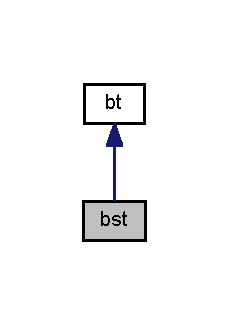
\includegraphics[width=110pt]{classbst__inherit__graph}
\end{center}
\end{figure}


Collaboration diagram for bst\-:
\nopagebreak
\begin{figure}[H]
\begin{center}
\leavevmode
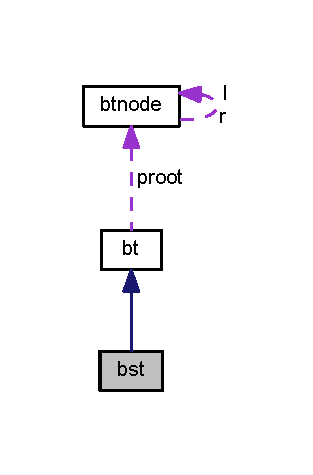
\includegraphics[width=150pt]{classbst__coll__graph}
\end{center}
\end{figure}
\subsection*{Public Member Functions}
\begin{DoxyCompactItemize}
\item 
\hyperlink{classbst_a7e853bf07e80d1ca3f63147ca056885b}{bst} ()
\item 
\hyperlink{classbst_ac2d09618fef6c8771b13126271658650}{bst} (int $\ast$p, int $\ast$q)
\item 
\hyperlink{classbst_ab8c59af54f80760f70af65da6d9ed0b5}{bst} (int $\ast$p, int size)
\item 
\hyperlink{classbst_ad1de95dd42e0b0f7e068067517807768}{bst} (const vector$<$ int $>$ \&v)
\item 
\hyperlink{classbst_a4755b663e678f2207dc32caccb5bb18d}{$\sim$bst} ()
\item 
void \hyperlink{classbst_a843b0fe1972a0008170abed11e5d3968}{insert} (int n)
\begin{DoxyCompactList}\small\item\em @ \end{DoxyCompactList}\item 
void \hyperlink{classbst_af96154a8371024bffc9f157e7cde2967}{insert} (int $\ast$p, int $\ast$q)
\item 
void \hyperlink{classbst_a2221f83ef688d5ae829502c77f16fce1}{insert} (int $\ast$p, int size)
\item 
void \hyperlink{classbst_ac5f3349098823cc08e76f22b7e3be371}{insert} (const vector$<$ int $>$ \&v)
\item 
vector$<$ int $>$ \hyperlink{classbst_a9e8eceb111915919599c147e2d3b9fb0}{walk} (\hyperlink{bst_8h_ae70daad8be95b143e7f97f55e1c4e743}{W\-A\-L\-K\-O\-R\-D\-E\-R} wo, bool norecursive=true) const 
\begin{DoxyCompactList}\small\item\em P\-O\-S\-T\-O\-R\-D\-E\-R is more complex than the other two traversals (due to its nature of non-\/tail recursion there is an extra statement after the final recursive call to itself). \end{DoxyCompactList}\item 
void \hyperlink{classbst_a698bfef73902a195688efcdc0aad32d4}{nullify} ()
\item 
size\-\_\-t \hyperlink{classbst_a891aa44765d452e600b6f1be79b1a7d6}{height} ()
\item 
size\-\_\-t \hyperlink{classbst_a24751e37cedacf3be3a09385df994690}{height\-\_\-min} ()
\item 
size\-\_\-t \hyperlink{classbst_abee0b512bbaf837d3a7abbbf2b4db1f7}{height\-\_\-max} ()
\item 
size\-\_\-t \hyperlink{classbst_a4d6ee35a495f93588fa9a9a1219550f4}{inbalance} ()
\end{DoxyCompactItemize}
\subsection*{Static Public Member Functions}
\begin{DoxyCompactItemize}
\item 
static bool \hyperlink{classbst_a09e7cdc8b9c0c097113de2ba2186c8aa}{is\-B\-S\-T} (const \hyperlink{classbst}{bst} \&t)
\item 
static \hyperlink{bst_8h_ae70daad8be95b143e7f97f55e1c4e743}{W\-A\-L\-K\-O\-R\-D\-E\-R} \hyperlink{classbst_a9359ae8d6b38050b3bc1afc76550a775}{get\-Order} (const vector$<$ int $>$ \&v)
\item 
static bool \hyperlink{classbst_a3d50d6acb133502be01a5ef75eae613d}{test} ()
\end{DoxyCompactItemize}
\subsection*{Additional Inherited Members}


\subsection{Detailed Description}
an binary search tree 

Definition at line 36 of file bst.\-h.



\subsection{Constructor \& Destructor Documentation}
\hypertarget{classbst_a7e853bf07e80d1ca3f63147ca056885b}{\index{bst@{bst}!bst@{bst}}
\index{bst@{bst}!bst@{bst}}
\subsubsection[{bst}]{\setlength{\rightskip}{0pt plus 5cm}bst\-::bst (
\begin{DoxyParamCaption}
{}
\end{DoxyParamCaption}
)}}\label{classbst_a7e853bf07e80d1ca3f63147ca056885b}


Definition at line 9 of file bst.\-cpp.

\hypertarget{classbst_ac2d09618fef6c8771b13126271658650}{\index{bst@{bst}!bst@{bst}}
\index{bst@{bst}!bst@{bst}}
\subsubsection[{bst}]{\setlength{\rightskip}{0pt plus 5cm}bst\-::bst (
\begin{DoxyParamCaption}
\item[{int $\ast$}]{p, }
\item[{int $\ast$}]{q}
\end{DoxyParamCaption}
)}}\label{classbst_ac2d09618fef6c8771b13126271658650}
\hypertarget{classbst_ab8c59af54f80760f70af65da6d9ed0b5}{\index{bst@{bst}!bst@{bst}}
\index{bst@{bst}!bst@{bst}}
\subsubsection[{bst}]{\setlength{\rightskip}{0pt plus 5cm}bst\-::bst (
\begin{DoxyParamCaption}
\item[{int $\ast$}]{p, }
\item[{int}]{size}
\end{DoxyParamCaption}
)}}\label{classbst_ab8c59af54f80760f70af65da6d9ed0b5}
\hypertarget{classbst_ad1de95dd42e0b0f7e068067517807768}{\index{bst@{bst}!bst@{bst}}
\index{bst@{bst}!bst@{bst}}
\subsubsection[{bst}]{\setlength{\rightskip}{0pt plus 5cm}bst\-::bst (
\begin{DoxyParamCaption}
\item[{const vector$<$ int $>$ \&}]{v}
\end{DoxyParamCaption}
)}}\label{classbst_ad1de95dd42e0b0f7e068067517807768}
\hypertarget{classbst_a4755b663e678f2207dc32caccb5bb18d}{\index{bst@{bst}!$\sim$bst@{$\sim$bst}}
\index{$\sim$bst@{$\sim$bst}!bst@{bst}}
\subsubsection[{$\sim$bst}]{\setlength{\rightskip}{0pt plus 5cm}bst\-::$\sim$bst (
\begin{DoxyParamCaption}
{}
\end{DoxyParamCaption}
)}}\label{classbst_a4755b663e678f2207dc32caccb5bb18d}


Definition at line 12 of file bst.\-cpp.



\subsection{Member Function Documentation}
\hypertarget{classbst_a9359ae8d6b38050b3bc1afc76550a775}{\index{bst@{bst}!get\-Order@{get\-Order}}
\index{get\-Order@{get\-Order}!bst@{bst}}
\subsubsection[{get\-Order}]{\setlength{\rightskip}{0pt plus 5cm}{\bf W\-A\-L\-K\-O\-R\-D\-E\-R} bst\-::get\-Order (
\begin{DoxyParamCaption}
\item[{const vector$<$ int $>$ \&}]{v}
\end{DoxyParamCaption}
)\hspace{0.3cm}{\ttfamily [static]}}}\label{classbst_a9359ae8d6b38050b3bc1afc76550a775}


Definition at line 246 of file bst.\-cpp.

\hypertarget{classbst_a891aa44765d452e600b6f1be79b1a7d6}{\index{bst@{bst}!height@{height}}
\index{height@{height}!bst@{bst}}
\subsubsection[{height}]{\setlength{\rightskip}{0pt plus 5cm}size\-\_\-t bst\-::height (
\begin{DoxyParamCaption}
{}
\end{DoxyParamCaption}
)}}\label{classbst_a891aa44765d452e600b6f1be79b1a7d6}
\hypertarget{classbst_abee0b512bbaf837d3a7abbbf2b4db1f7}{\index{bst@{bst}!height\-\_\-max@{height\-\_\-max}}
\index{height\-\_\-max@{height\-\_\-max}!bst@{bst}}
\subsubsection[{height\-\_\-max}]{\setlength{\rightskip}{0pt plus 5cm}size\-\_\-t bst\-::height\-\_\-max (
\begin{DoxyParamCaption}
{}
\end{DoxyParamCaption}
)}}\label{classbst_abee0b512bbaf837d3a7abbbf2b4db1f7}
\hypertarget{classbst_a24751e37cedacf3be3a09385df994690}{\index{bst@{bst}!height\-\_\-min@{height\-\_\-min}}
\index{height\-\_\-min@{height\-\_\-min}!bst@{bst}}
\subsubsection[{height\-\_\-min}]{\setlength{\rightskip}{0pt plus 5cm}size\-\_\-t bst\-::height\-\_\-min (
\begin{DoxyParamCaption}
{}
\end{DoxyParamCaption}
)}}\label{classbst_a24751e37cedacf3be3a09385df994690}
\hypertarget{classbst_a4d6ee35a495f93588fa9a9a1219550f4}{\index{bst@{bst}!inbalance@{inbalance}}
\index{inbalance@{inbalance}!bst@{bst}}
\subsubsection[{inbalance}]{\setlength{\rightskip}{0pt plus 5cm}size\-\_\-t bst\-::inbalance (
\begin{DoxyParamCaption}
{}
\end{DoxyParamCaption}
)}}\label{classbst_a4d6ee35a495f93588fa9a9a1219550f4}
\hypertarget{classbst_a843b0fe1972a0008170abed11e5d3968}{\index{bst@{bst}!insert@{insert}}
\index{insert@{insert}!bst@{bst}}
\subsubsection[{insert}]{\setlength{\rightskip}{0pt plus 5cm}void bst\-::insert (
\begin{DoxyParamCaption}
\item[{int}]{n}
\end{DoxyParamCaption}
)}}\label{classbst_a843b0fe1972a0008170abed11e5d3968}


@ 



Definition at line 17 of file bst.\-cpp.



Here is the caller graph for this function\-:
\nopagebreak
\begin{figure}[H]
\begin{center}
\leavevmode
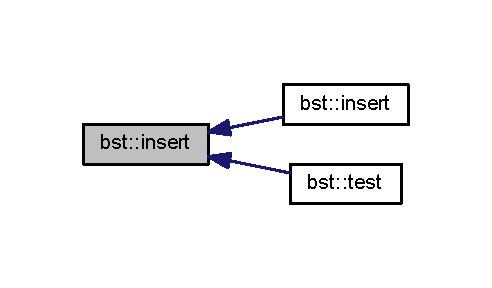
\includegraphics[width=236pt]{classbst_a843b0fe1972a0008170abed11e5d3968_icgraph}
\end{center}
\end{figure}


\hypertarget{classbst_af96154a8371024bffc9f157e7cde2967}{\index{bst@{bst}!insert@{insert}}
\index{insert@{insert}!bst@{bst}}
\subsubsection[{insert}]{\setlength{\rightskip}{0pt plus 5cm}void bst\-::insert (
\begin{DoxyParamCaption}
\item[{int $\ast$}]{p, }
\item[{int $\ast$}]{q}
\end{DoxyParamCaption}
)}}\label{classbst_af96154a8371024bffc9f157e7cde2967}


Definition at line 45 of file bst.\-cpp.



Here is the call graph for this function\-:
\nopagebreak
\begin{figure}[H]
\begin{center}
\leavevmode
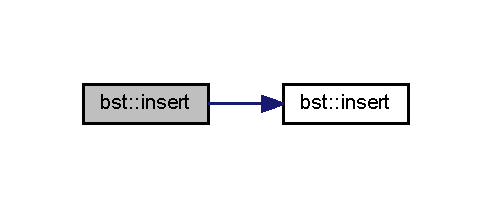
\includegraphics[width=236pt]{classbst_af96154a8371024bffc9f157e7cde2967_cgraph}
\end{center}
\end{figure}


\hypertarget{classbst_a2221f83ef688d5ae829502c77f16fce1}{\index{bst@{bst}!insert@{insert}}
\index{insert@{insert}!bst@{bst}}
\subsubsection[{insert}]{\setlength{\rightskip}{0pt plus 5cm}void bst\-::insert (
\begin{DoxyParamCaption}
\item[{int $\ast$}]{p, }
\item[{int}]{size}
\end{DoxyParamCaption}
)}}\label{classbst_a2221f83ef688d5ae829502c77f16fce1}


Definition at line 53 of file bst.\-cpp.



Here is the call graph for this function\-:
\nopagebreak
\begin{figure}[H]
\begin{center}
\leavevmode
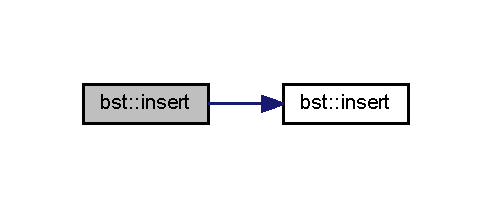
\includegraphics[width=236pt]{classbst_a2221f83ef688d5ae829502c77f16fce1_cgraph}
\end{center}
\end{figure}


\hypertarget{classbst_ac5f3349098823cc08e76f22b7e3be371}{\index{bst@{bst}!insert@{insert}}
\index{insert@{insert}!bst@{bst}}
\subsubsection[{insert}]{\setlength{\rightskip}{0pt plus 5cm}void bst\-::insert (
\begin{DoxyParamCaption}
\item[{const vector$<$ int $>$ \&}]{v}
\end{DoxyParamCaption}
)}}\label{classbst_ac5f3349098823cc08e76f22b7e3be371}


Definition at line 61 of file bst.\-cpp.



Here is the call graph for this function\-:
\nopagebreak
\begin{figure}[H]
\begin{center}
\leavevmode
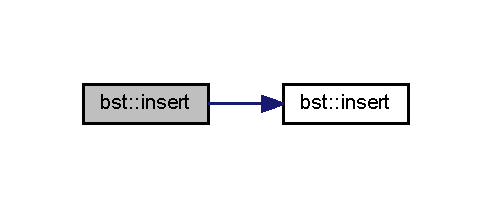
\includegraphics[width=236pt]{classbst_ac5f3349098823cc08e76f22b7e3be371_cgraph}
\end{center}
\end{figure}


\hypertarget{classbst_a09e7cdc8b9c0c097113de2ba2186c8aa}{\index{bst@{bst}!is\-B\-S\-T@{is\-B\-S\-T}}
\index{is\-B\-S\-T@{is\-B\-S\-T}!bst@{bst}}
\subsubsection[{is\-B\-S\-T}]{\setlength{\rightskip}{0pt plus 5cm}bool bst\-::is\-B\-S\-T (
\begin{DoxyParamCaption}
\item[{const {\bf bst} \&}]{t}
\end{DoxyParamCaption}
)\hspace{0.3cm}{\ttfamily [static]}}}\label{classbst_a09e7cdc8b9c0c097113de2ba2186c8aa}


Definition at line 233 of file bst.\-cpp.



Here is the call graph for this function\-:
\nopagebreak
\begin{figure}[H]
\begin{center}
\leavevmode
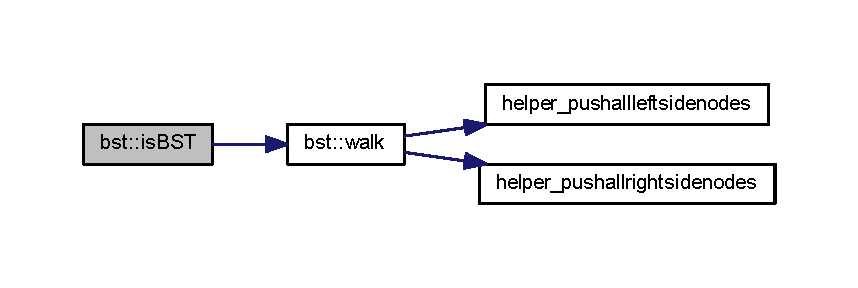
\includegraphics[width=350pt]{classbst_a09e7cdc8b9c0c097113de2ba2186c8aa_cgraph}
\end{center}
\end{figure}




Here is the caller graph for this function\-:
\nopagebreak
\begin{figure}[H]
\begin{center}
\leavevmode
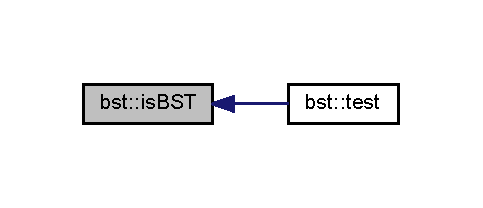
\includegraphics[width=232pt]{classbst_a09e7cdc8b9c0c097113de2ba2186c8aa_icgraph}
\end{center}
\end{figure}


\hypertarget{classbst_a698bfef73902a195688efcdc0aad32d4}{\index{bst@{bst}!nullify@{nullify}}
\index{nullify@{nullify}!bst@{bst}}
\subsubsection[{nullify}]{\setlength{\rightskip}{0pt plus 5cm}void bst\-::nullify (
\begin{DoxyParamCaption}
{}
\end{DoxyParamCaption}
)}}\label{classbst_a698bfef73902a195688efcdc0aad32d4}
\hypertarget{classbst_a3d50d6acb133502be01a5ef75eae613d}{\index{bst@{bst}!test@{test}}
\index{test@{test}!bst@{bst}}
\subsubsection[{test}]{\setlength{\rightskip}{0pt plus 5cm}bool bst\-::test (
\begin{DoxyParamCaption}
{}
\end{DoxyParamCaption}
)\hspace{0.3cm}{\ttfamily [static]}}}\label{classbst_a3d50d6acb133502be01a5ef75eae613d}


Definition at line 250 of file bst.\-cpp.



Here is the call graph for this function\-:
\nopagebreak
\begin{figure}[H]
\begin{center}
\leavevmode
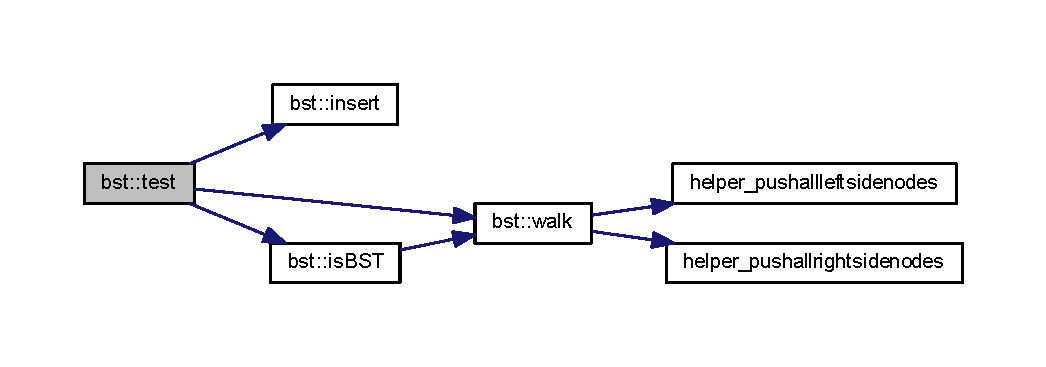
\includegraphics[width=350pt]{classbst_a3d50d6acb133502be01a5ef75eae613d_cgraph}
\end{center}
\end{figure}


\hypertarget{classbst_a9e8eceb111915919599c147e2d3b9fb0}{\index{bst@{bst}!walk@{walk}}
\index{walk@{walk}!bst@{bst}}
\subsubsection[{walk}]{\setlength{\rightskip}{0pt plus 5cm}vector$<$ int $>$ bst\-::walk (
\begin{DoxyParamCaption}
\item[{{\bf W\-A\-L\-K\-O\-R\-D\-E\-R}}]{wo, }
\item[{bool}]{norecursive = {\ttfamily true}}
\end{DoxyParamCaption}
) const}}\label{classbst_a9e8eceb111915919599c147e2d3b9fb0}


P\-O\-S\-T\-O\-R\-D\-E\-R is more complex than the other two traversals (due to its nature of non-\/tail recursion there is an extra statement after the final recursive call to itself). 



Definition at line 136 of file bst.\-cpp.



Here is the call graph for this function\-:
\nopagebreak
\begin{figure}[H]
\begin{center}
\leavevmode
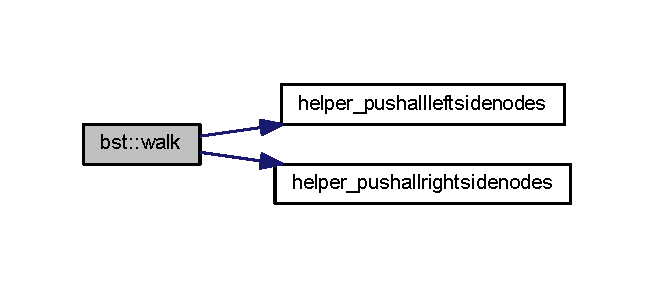
\includegraphics[width=314pt]{classbst_a9e8eceb111915919599c147e2d3b9fb0_cgraph}
\end{center}
\end{figure}




Here is the caller graph for this function\-:
\nopagebreak
\begin{figure}[H]
\begin{center}
\leavevmode
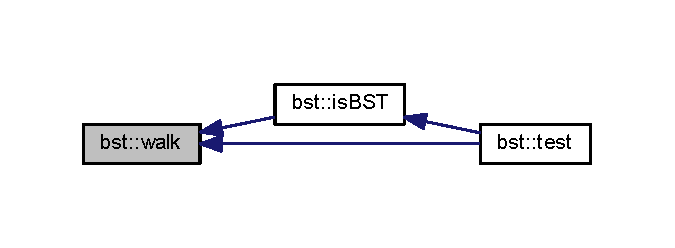
\includegraphics[width=324pt]{classbst_a9e8eceb111915919599c147e2d3b9fb0_icgraph}
\end{center}
\end{figure}




The documentation for this class was generated from the following files\-:\begin{DoxyCompactItemize}
\item 
Algo/\hyperlink{bst_8h}{bst.\-h}\item 
Algo/\hyperlink{bst_8cpp}{bst.\-cpp}\end{DoxyCompactItemize}

\hypertarget{classbt}{\section{bt Class Reference}
\label{classbt}\index{bt@{bt}}
}


an arbitrary binary tree  




{\ttfamily \#include $<$bst.\-h$>$}



Inheritance diagram for bt\-:
\nopagebreak
\begin{figure}[H]
\begin{center}
\leavevmode
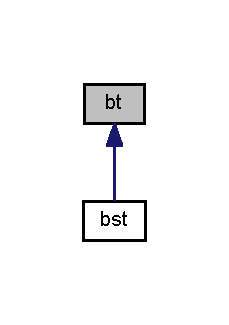
\includegraphics[width=110pt]{classbt__inherit__graph}
\end{center}
\end{figure}


Collaboration diagram for bt\-:
\nopagebreak
\begin{figure}[H]
\begin{center}
\leavevmode
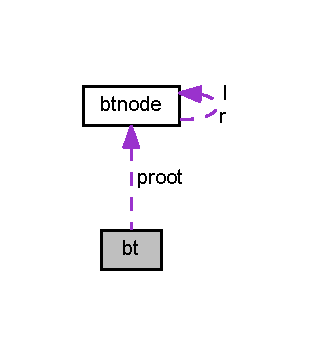
\includegraphics[width=150pt]{classbt__coll__graph}
\end{center}
\end{figure}
\subsection*{Public Member Functions}
\begin{DoxyCompactItemize}
\item 
\hyperlink{classbt_a39717d66f405aeb141610d4c8854c583}{bt} ()
\end{DoxyCompactItemize}
\subsection*{Protected Attributes}
\begin{DoxyCompactItemize}
\item 
\hyperlink{structbtnode}{btnode} $\ast$ \hyperlink{classbt_ad13cd5d42935ee352fb82b7d96368db6}{proot}
\end{DoxyCompactItemize}


\subsection{Detailed Description}
an arbitrary binary tree 

Definition at line 19 of file bst.\-h.



\subsection{Constructor \& Destructor Documentation}
\hypertarget{classbt_a39717d66f405aeb141610d4c8854c583}{\index{bt@{bt}!bt@{bt}}
\index{bt@{bt}!bt@{bt}}
\subsubsection[{bt}]{\setlength{\rightskip}{0pt plus 5cm}bt\-::bt (
\begin{DoxyParamCaption}
{}
\end{DoxyParamCaption}
)\hspace{0.3cm}{\ttfamily [inline]}}}\label{classbt_a39717d66f405aeb141610d4c8854c583}


Definition at line 23 of file bst.\-h.



\subsection{Member Data Documentation}
\hypertarget{classbt_ad13cd5d42935ee352fb82b7d96368db6}{\index{bt@{bt}!proot@{proot}}
\index{proot@{proot}!bt@{bt}}
\subsubsection[{proot}]{\setlength{\rightskip}{0pt plus 5cm}{\bf btnode}$\ast$ bt\-::proot\hspace{0.3cm}{\ttfamily [protected]}}}\label{classbt_ad13cd5d42935ee352fb82b7d96368db6}


Definition at line 21 of file bst.\-h.



The documentation for this class was generated from the following file\-:\begin{DoxyCompactItemize}
\item 
Algo/\hyperlink{bst_8h}{bst.\-h}\end{DoxyCompactItemize}

\hypertarget{structbtnode}{\section{btnode Struct Reference}
\label{structbtnode}\index{btnode@{btnode}}
}


arbitrary binary tree node\mbox{[}bst,heap,etc\mbox{]}  




{\ttfamily \#include $<$bst.\-h$>$}



Collaboration diagram for btnode\-:
\nopagebreak
\begin{figure}[H]
\begin{center}
\leavevmode
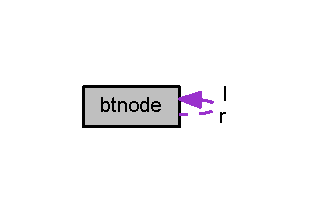
\includegraphics[width=150pt]{structbtnode__coll__graph}
\end{center}
\end{figure}
\subsection*{Public Member Functions}
\begin{DoxyCompactItemize}
\item 
\hyperlink{structbtnode_aa500392cc9dbda127e5cd1ff1297bdfa}{btnode} (int n)
\end{DoxyCompactItemize}
\subsection*{Public Attributes}
\begin{DoxyCompactItemize}
\item 
\hyperlink{structbtnode}{btnode} $\ast$ \hyperlink{structbtnode_af6ef69a154018945fa5e1a5287dfc4e0}{l}
\item 
\hyperlink{structbtnode}{btnode} $\ast$ \hyperlink{structbtnode_aad4b4a959992763c35c51f313c698002}{r}
\item 
int \hyperlink{structbtnode_aa78fe8dab99932fc364224bc83524771}{d}
\item 
short \hyperlink{structbtnode_a8cac175e3c667951b9346559f291da16}{color}
\end{DoxyCompactItemize}


\subsection{Detailed Description}
arbitrary binary tree node\mbox{[}bst,heap,etc\mbox{]} 

Definition at line 10 of file bst.\-h.



\subsection{Constructor \& Destructor Documentation}
\hypertarget{structbtnode_aa500392cc9dbda127e5cd1ff1297bdfa}{\index{btnode@{btnode}!btnode@{btnode}}
\index{btnode@{btnode}!btnode@{btnode}}
\subsubsection[{btnode}]{\setlength{\rightskip}{0pt plus 5cm}btnode\-::btnode (
\begin{DoxyParamCaption}
\item[{int}]{n}
\end{DoxyParamCaption}
)\hspace{0.3cm}{\ttfamily [inline]}}}\label{structbtnode_aa500392cc9dbda127e5cd1ff1297bdfa}


Definition at line 15 of file bst.\-h.



\subsection{Member Data Documentation}
\hypertarget{structbtnode_a8cac175e3c667951b9346559f291da16}{\index{btnode@{btnode}!color@{color}}
\index{color@{color}!btnode@{btnode}}
\subsubsection[{color}]{\setlength{\rightskip}{0pt plus 5cm}short btnode\-::color}}\label{structbtnode_a8cac175e3c667951b9346559f291da16}


Definition at line 14 of file bst.\-h.

\hypertarget{structbtnode_aa78fe8dab99932fc364224bc83524771}{\index{btnode@{btnode}!d@{d}}
\index{d@{d}!btnode@{btnode}}
\subsubsection[{d}]{\setlength{\rightskip}{0pt plus 5cm}int btnode\-::d}}\label{structbtnode_aa78fe8dab99932fc364224bc83524771}


Definition at line 13 of file bst.\-h.

\hypertarget{structbtnode_af6ef69a154018945fa5e1a5287dfc4e0}{\index{btnode@{btnode}!l@{l}}
\index{l@{l}!btnode@{btnode}}
\subsubsection[{l}]{\setlength{\rightskip}{0pt plus 5cm}{\bf btnode}$\ast$ btnode\-::l}}\label{structbtnode_af6ef69a154018945fa5e1a5287dfc4e0}


Definition at line 11 of file bst.\-h.

\hypertarget{structbtnode_aad4b4a959992763c35c51f313c698002}{\index{btnode@{btnode}!r@{r}}
\index{r@{r}!btnode@{btnode}}
\subsubsection[{r}]{\setlength{\rightskip}{0pt plus 5cm}{\bf btnode}$\ast$ btnode\-::r}}\label{structbtnode_aad4b4a959992763c35c51f313c698002}


Definition at line 12 of file bst.\-h.



The documentation for this struct was generated from the following file\-:\begin{DoxyCompactItemize}
\item 
Algo/\hyperlink{bst_8h}{bst.\-h}\end{DoxyCompactItemize}

\hypertarget{classdclist}{\section{dclist Class Reference}
\label{classdclist}\index{dclist@{dclist}}
}


A Circular Double Linked List.  




{\ttfamily \#include $<$list.\-h$>$}

\subsection*{Public Member Functions}
\begin{DoxyCompactItemize}
\item 
\hyperlink{classdclist_adf50f8c57c3fd39aabf60fad51033c0e}{dclist} ()
\item 
\hyperlink{classdclist_a7eec5a55914fb005e39bf0f09ea938ba}{dclist} (int $\ast$p, int $\ast$q)
\item 
\hyperlink{classdclist_a7f87e0b8b308dd3fe0c3b8017aad2973}{dclist} (int $\ast$p, int \hyperlink{classdclist_a4aad3140e1ecd8f9ae393cfe42b440a5}{size})
\item 
\hyperlink{classdclist_a7f3da5d5f4ede734c5cbe7b2ecd31980}{dclist} (const vector$<$ int $>$ \&v)
\item 
\hyperlink{classdclist_a42c10662b1c0b0c5d91236a10aacc638}{$\sim$dclist} ()
\item 
\hyperlink{structdlist__node}{dlist\-\_\-node} $\ast$ \hyperlink{classdclist_a02c4135f1d4bfd026e2634ce97e11bc2}{end} ()
\begin{DoxyCompactList}\small\item\em pass the end, which is the same as the sentinel in this case \end{DoxyCompactList}\item 
\hyperlink{structdlist__node}{dlist\-\_\-node} $\ast$ \hyperlink{classdclist_a04e5f7c6204e24ab0bbcb6d9cf732301}{begin} ()
\item 
size\-\_\-t \hyperlink{classdclist_a4aad3140e1ecd8f9ae393cfe42b440a5}{size} ()
\item 
void \hyperlink{classdclist_a8137b2afc567b71225b97ebe32de6ea8}{push\-\_\-front} (int n)
\begin{DoxyCompactList}\small\item\em push new node as the next of sentinel \end{DoxyCompactList}\item 
void \hyperlink{classdclist_ac7c566527b54091161415781db391d27}{push\-\_\-front} (int $\ast$p, int $\ast$q)
\item 
void \hyperlink{classdclist_a6c338aa455d29ae6ce6d8011e5e1586b}{push\-\_\-end} (int n)
\begin{DoxyCompactList}\small\item\em push new node as the previous of sentinel\par
 A.\-next=B then B.\-prev=A, they always appear as a pair \end{DoxyCompactList}\item 
void \hyperlink{classdclist_a84bde4e87316ce56868823c5f4513b8a}{reverse} ()
\begin{DoxyCompactList}\small\item\em swap pointer prev and next for every node including sentinel \end{DoxyCompactList}\end{DoxyCompactItemize}
\subsection*{Static Public Member Functions}
\begin{DoxyCompactItemize}
\item 
static bool \hyperlink{classdclist_ac1dd6df031caf8994d688aca88ba09d3}{test} ()
\end{DoxyCompactItemize}


\subsection{Detailed Description}
A Circular Double Linked List. 

Definition at line 61 of file list.\-h.



\subsection{Constructor \& Destructor Documentation}
\hypertarget{classdclist_adf50f8c57c3fd39aabf60fad51033c0e}{\index{dclist@{dclist}!dclist@{dclist}}
\index{dclist@{dclist}!dclist@{dclist}}
\subsubsection[{dclist}]{\setlength{\rightskip}{0pt plus 5cm}dclist\-::dclist (
\begin{DoxyParamCaption}
{}
\end{DoxyParamCaption}
)}}\label{classdclist_adf50f8c57c3fd39aabf60fad51033c0e}


Definition at line 11 of file dlist.\-cpp.

\hypertarget{classdclist_a7eec5a55914fb005e39bf0f09ea938ba}{\index{dclist@{dclist}!dclist@{dclist}}
\index{dclist@{dclist}!dclist@{dclist}}
\subsubsection[{dclist}]{\setlength{\rightskip}{0pt plus 5cm}dclist\-::dclist (
\begin{DoxyParamCaption}
\item[{int $\ast$}]{p, }
\item[{int $\ast$}]{q}
\end{DoxyParamCaption}
)}}\label{classdclist_a7eec5a55914fb005e39bf0f09ea938ba}


Definition at line 15 of file dlist.\-cpp.



Here is the call graph for this function\-:
\nopagebreak
\begin{figure}[H]
\begin{center}
\leavevmode
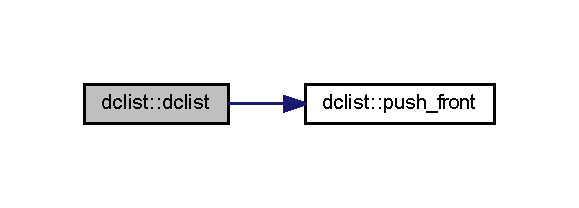
\includegraphics[width=278pt]{classdclist_a7eec5a55914fb005e39bf0f09ea938ba_cgraph}
\end{center}
\end{figure}


\hypertarget{classdclist_a7f87e0b8b308dd3fe0c3b8017aad2973}{\index{dclist@{dclist}!dclist@{dclist}}
\index{dclist@{dclist}!dclist@{dclist}}
\subsubsection[{dclist}]{\setlength{\rightskip}{0pt plus 5cm}dclist\-::dclist (
\begin{DoxyParamCaption}
\item[{int $\ast$}]{p, }
\item[{int}]{size}
\end{DoxyParamCaption}
)}}\label{classdclist_a7f87e0b8b308dd3fe0c3b8017aad2973}


Definition at line 20 of file dlist.\-cpp.

\hypertarget{classdclist_a7f3da5d5f4ede734c5cbe7b2ecd31980}{\index{dclist@{dclist}!dclist@{dclist}}
\index{dclist@{dclist}!dclist@{dclist}}
\subsubsection[{dclist}]{\setlength{\rightskip}{0pt plus 5cm}dclist\-::dclist (
\begin{DoxyParamCaption}
\item[{const vector$<$ int $>$ \&}]{v}
\end{DoxyParamCaption}
)}}\label{classdclist_a7f3da5d5f4ede734c5cbe7b2ecd31980}


Definition at line 24 of file dlist.\-cpp.

\hypertarget{classdclist_a42c10662b1c0b0c5d91236a10aacc638}{\index{dclist@{dclist}!$\sim$dclist@{$\sim$dclist}}
\index{$\sim$dclist@{$\sim$dclist}!dclist@{dclist}}
\subsubsection[{$\sim$dclist}]{\setlength{\rightskip}{0pt plus 5cm}dclist\-::$\sim$dclist (
\begin{DoxyParamCaption}
{}
\end{DoxyParamCaption}
)}}\label{classdclist_a42c10662b1c0b0c5d91236a10aacc638}


Definition at line 28 of file dlist.\-cpp.



\subsection{Member Function Documentation}
\hypertarget{classdclist_a04e5f7c6204e24ab0bbcb6d9cf732301}{\index{dclist@{dclist}!begin@{begin}}
\index{begin@{begin}!dclist@{dclist}}
\subsubsection[{begin}]{\setlength{\rightskip}{0pt plus 5cm}{\bf dlist\-\_\-node} $\ast$ dclist\-::begin (
\begin{DoxyParamCaption}
{}
\end{DoxyParamCaption}
)}}\label{classdclist_a04e5f7c6204e24ab0bbcb6d9cf732301}


Definition at line 38 of file dlist.\-cpp.



Here is the caller graph for this function\-:
\nopagebreak
\begin{figure}[H]
\begin{center}
\leavevmode
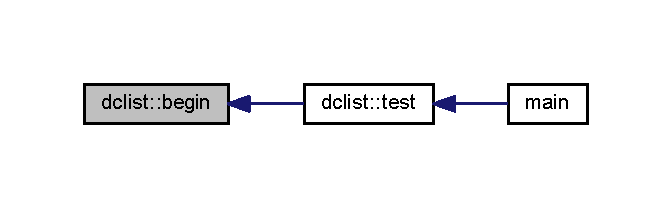
\includegraphics[width=322pt]{classdclist_a04e5f7c6204e24ab0bbcb6d9cf732301_icgraph}
\end{center}
\end{figure}


\hypertarget{classdclist_a02c4135f1d4bfd026e2634ce97e11bc2}{\index{dclist@{dclist}!end@{end}}
\index{end@{end}!dclist@{dclist}}
\subsubsection[{end}]{\setlength{\rightskip}{0pt plus 5cm}{\bf dlist\-\_\-node} $\ast$ dclist\-::end (
\begin{DoxyParamCaption}
{}
\end{DoxyParamCaption}
)}}\label{classdclist_a02c4135f1d4bfd026e2634ce97e11bc2}


pass the end, which is the same as the sentinel in this case 



Definition at line 34 of file dlist.\-cpp.



Here is the caller graph for this function\-:
\nopagebreak
\begin{figure}[H]
\begin{center}
\leavevmode
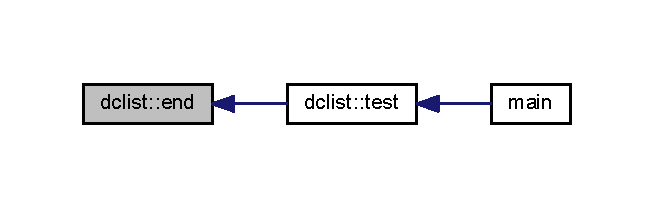
\includegraphics[width=314pt]{classdclist_a02c4135f1d4bfd026e2634ce97e11bc2_icgraph}
\end{center}
\end{figure}


\hypertarget{classdclist_a6c338aa455d29ae6ce6d8011e5e1586b}{\index{dclist@{dclist}!push\-\_\-end@{push\-\_\-end}}
\index{push\-\_\-end@{push\-\_\-end}!dclist@{dclist}}
\subsubsection[{push\-\_\-end}]{\setlength{\rightskip}{0pt plus 5cm}void dclist\-::push\-\_\-end (
\begin{DoxyParamCaption}
\item[{int}]{n}
\end{DoxyParamCaption}
)}}\label{classdclist_a6c338aa455d29ae6ce6d8011e5e1586b}


push new node as the previous of sentinel\par
 A.\-next=B then B.\-prev=A, they always appear as a pair 



Definition at line 70 of file dlist.\-cpp.

\hypertarget{classdclist_a8137b2afc567b71225b97ebe32de6ea8}{\index{dclist@{dclist}!push\-\_\-front@{push\-\_\-front}}
\index{push\-\_\-front@{push\-\_\-front}!dclist@{dclist}}
\subsubsection[{push\-\_\-front}]{\setlength{\rightskip}{0pt plus 5cm}void dclist\-::push\-\_\-front (
\begin{DoxyParamCaption}
\item[{int}]{n}
\end{DoxyParamCaption}
)}}\label{classdclist_a8137b2afc567b71225b97ebe32de6ea8}


push new node as the next of sentinel 



Definition at line 47 of file dlist.\-cpp.



Here is the caller graph for this function\-:
\nopagebreak
\begin{figure}[H]
\begin{center}
\leavevmode
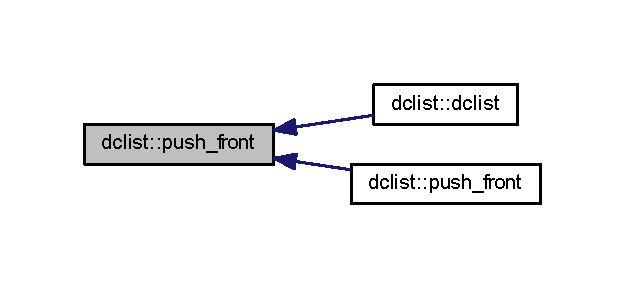
\includegraphics[width=300pt]{classdclist_a8137b2afc567b71225b97ebe32de6ea8_icgraph}
\end{center}
\end{figure}


\hypertarget{classdclist_ac7c566527b54091161415781db391d27}{\index{dclist@{dclist}!push\-\_\-front@{push\-\_\-front}}
\index{push\-\_\-front@{push\-\_\-front}!dclist@{dclist}}
\subsubsection[{push\-\_\-front}]{\setlength{\rightskip}{0pt plus 5cm}void dclist\-::push\-\_\-front (
\begin{DoxyParamCaption}
\item[{int $\ast$}]{p, }
\item[{int $\ast$}]{q}
\end{DoxyParamCaption}
)}}\label{classdclist_ac7c566527b54091161415781db391d27}


Definition at line 61 of file dlist.\-cpp.



Here is the call graph for this function\-:
\nopagebreak
\begin{figure}[H]
\begin{center}
\leavevmode
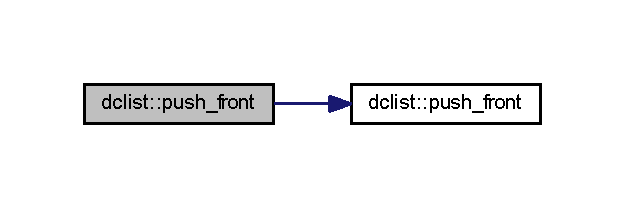
\includegraphics[width=300pt]{classdclist_ac7c566527b54091161415781db391d27_cgraph}
\end{center}
\end{figure}


\hypertarget{classdclist_a84bde4e87316ce56868823c5f4513b8a}{\index{dclist@{dclist}!reverse@{reverse}}
\index{reverse@{reverse}!dclist@{dclist}}
\subsubsection[{reverse}]{\setlength{\rightskip}{0pt plus 5cm}void dclist\-::reverse (
\begin{DoxyParamCaption}
{}
\end{DoxyParamCaption}
)}}\label{classdclist_a84bde4e87316ce56868823c5f4513b8a}


swap pointer prev and next for every node including sentinel 



Definition at line 84 of file dlist.\-cpp.



Here is the caller graph for this function\-:
\nopagebreak
\begin{figure}[H]
\begin{center}
\leavevmode
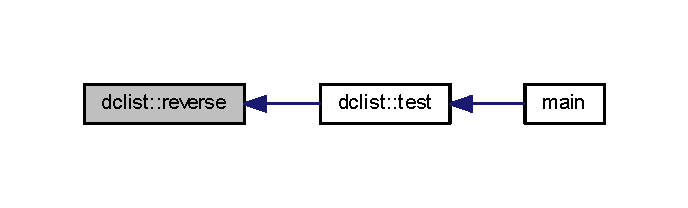
\includegraphics[width=330pt]{classdclist_a84bde4e87316ce56868823c5f4513b8a_icgraph}
\end{center}
\end{figure}


\hypertarget{classdclist_a4aad3140e1ecd8f9ae393cfe42b440a5}{\index{dclist@{dclist}!size@{size}}
\index{size@{size}!dclist@{dclist}}
\subsubsection[{size}]{\setlength{\rightskip}{0pt plus 5cm}size\-\_\-t dclist\-::size (
\begin{DoxyParamCaption}
{}
\end{DoxyParamCaption}
)}}\label{classdclist_a4aad3140e1ecd8f9ae393cfe42b440a5}


Definition at line 42 of file dlist.\-cpp.

\hypertarget{classdclist_ac1dd6df031caf8994d688aca88ba09d3}{\index{dclist@{dclist}!test@{test}}
\index{test@{test}!dclist@{dclist}}
\subsubsection[{test}]{\setlength{\rightskip}{0pt plus 5cm}bool dclist\-::test (
\begin{DoxyParamCaption}
{}
\end{DoxyParamCaption}
)\hspace{0.3cm}{\ttfamily [static]}}}\label{classdclist_ac1dd6df031caf8994d688aca88ba09d3}


Definition at line 93 of file dlist.\-cpp.



Here is the call graph for this function\-:
\nopagebreak
\begin{figure}[H]
\begin{center}
\leavevmode
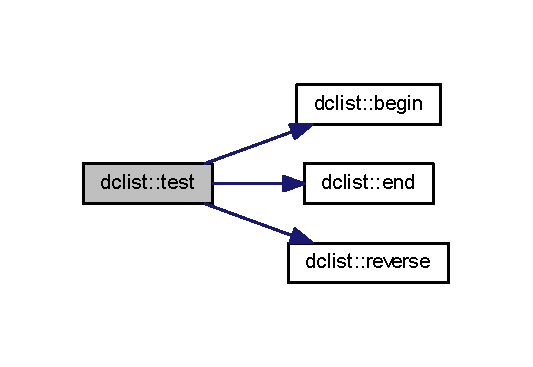
\includegraphics[width=256pt]{classdclist_ac1dd6df031caf8994d688aca88ba09d3_cgraph}
\end{center}
\end{figure}




Here is the caller graph for this function\-:
\nopagebreak
\begin{figure}[H]
\begin{center}
\leavevmode
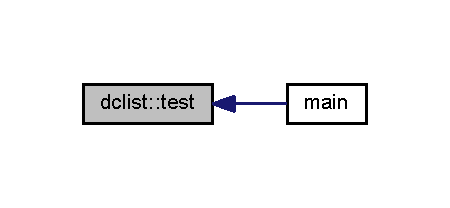
\includegraphics[width=216pt]{classdclist_ac1dd6df031caf8994d688aca88ba09d3_icgraph}
\end{center}
\end{figure}




The documentation for this class was generated from the following files\-:\begin{DoxyCompactItemize}
\item 
Algo/\hyperlink{list_8h}{list.\-h}\item 
Algo/\hyperlink{dlist_8cpp}{dlist.\-cpp}\end{DoxyCompactItemize}

\hypertarget{classdlist}{\section{dlist Class Reference}
\label{classdlist}\index{dlist@{dlist}}
}


A H\-E\-A\-D\-\_\-\-T\-A\-I\-L Double Linked List.  




{\ttfamily \#include $<$list.\-h$>$}

\subsection*{Public Member Functions}
\begin{DoxyCompactItemize}
\item 
\hyperlink{classdlist_a663ac3a48e3d2b426ca2c9a6ee091af3}{dlist} ()
\item 
\hyperlink{classdlist_ab185b9b5e9ff48e7f2f1e3a02af30cfd}{dlist} (int $\ast$p, int $\ast$q)
\item 
\hyperlink{classdlist_a70f123b97444609b43afcaa13153fd8b}{dlist} (int $\ast$p, int \hyperlink{classdlist_a426b9acc0f63b01e5f4551da5c7f1b84}{size})
\item 
\hyperlink{classdlist_ab63bbbb092e126601d75169a60457c04}{dlist} (const vector$<$ int $>$ \&v)
\item 
\hyperlink{classdlist_a5636a21a46af659872820e5bd12b0147}{$\sim$dlist} ()
\item 
\hyperlink{structdlist__node}{dlist\-\_\-node} $\ast$ \hyperlink{classdlist_a1e591a17f27f9b24eec115f5d74cc8d6}{end} ()
\begin{DoxyCompactList}\small\item\em pass the end, which is the same as the sentinel in this case \end{DoxyCompactList}\item 
\hyperlink{structdlist__node}{dlist\-\_\-node} $\ast$ \hyperlink{classdlist_ab8c324da167de0651de38d8302b790fd}{begin} ()
\item 
size\-\_\-t \hyperlink{classdlist_a426b9acc0f63b01e5f4551da5c7f1b84}{size} ()
\item 
void \hyperlink{classdlist_a0e57be4acd4778e5e97acafe702d265d}{push\-\_\-front} (int n)
\begin{DoxyCompactList}\small\item\em push new node as the next of sentinel \end{DoxyCompactList}\item 
void \hyperlink{classdlist_a04759f7a2f3e9026ab1bd17ba44261af}{push\-\_\-front} (int $\ast$p, int $\ast$q)
\item 
void \hyperlink{classdlist_a8b296336bec13013bc4068b2d5285e73}{push\-\_\-end} (int n)
\begin{DoxyCompactList}\small\item\em push new node as the previous of sentinel\par
 A.\-next=B then B.\-prev=A, they always appear as a pair \end{DoxyCompactList}\item 
void \hyperlink{classdlist_aec0249d97bef78564429292903a5a331}{reverse} ()
\begin{DoxyCompactList}\small\item\em swap pointer prev and next for every node including sentinel \end{DoxyCompactList}\end{DoxyCompactItemize}
\subsection*{Static Public Member Functions}
\begin{DoxyCompactItemize}
\item 
static void \hyperlink{classdlist_a4939b60463b87c6097dd8d098e2f4b52}{test} ()
\end{DoxyCompactItemize}


\subsection{Detailed Description}
A H\-E\-A\-D\-\_\-\-T\-A\-I\-L Double Linked List. 

Definition at line 24 of file list.\-h.



\subsection{Constructor \& Destructor Documentation}
\hypertarget{classdlist_a663ac3a48e3d2b426ca2c9a6ee091af3}{\index{dlist@{dlist}!dlist@{dlist}}
\index{dlist@{dlist}!dlist@{dlist}}
\subsubsection[{dlist}]{\setlength{\rightskip}{0pt plus 5cm}dlist\-::dlist (
\begin{DoxyParamCaption}
{}
\end{DoxyParamCaption}
)}}\label{classdlist_a663ac3a48e3d2b426ca2c9a6ee091af3}
\hypertarget{classdlist_ab185b9b5e9ff48e7f2f1e3a02af30cfd}{\index{dlist@{dlist}!dlist@{dlist}}
\index{dlist@{dlist}!dlist@{dlist}}
\subsubsection[{dlist}]{\setlength{\rightskip}{0pt plus 5cm}dlist\-::dlist (
\begin{DoxyParamCaption}
\item[{int $\ast$}]{p, }
\item[{int $\ast$}]{q}
\end{DoxyParamCaption}
)}}\label{classdlist_ab185b9b5e9ff48e7f2f1e3a02af30cfd}
\hypertarget{classdlist_a70f123b97444609b43afcaa13153fd8b}{\index{dlist@{dlist}!dlist@{dlist}}
\index{dlist@{dlist}!dlist@{dlist}}
\subsubsection[{dlist}]{\setlength{\rightskip}{0pt plus 5cm}dlist\-::dlist (
\begin{DoxyParamCaption}
\item[{int $\ast$}]{p, }
\item[{int}]{size}
\end{DoxyParamCaption}
)}}\label{classdlist_a70f123b97444609b43afcaa13153fd8b}
\hypertarget{classdlist_ab63bbbb092e126601d75169a60457c04}{\index{dlist@{dlist}!dlist@{dlist}}
\index{dlist@{dlist}!dlist@{dlist}}
\subsubsection[{dlist}]{\setlength{\rightskip}{0pt plus 5cm}dlist\-::dlist (
\begin{DoxyParamCaption}
\item[{const vector$<$ int $>$ \&}]{v}
\end{DoxyParamCaption}
)}}\label{classdlist_ab63bbbb092e126601d75169a60457c04}
\hypertarget{classdlist_a5636a21a46af659872820e5bd12b0147}{\index{dlist@{dlist}!$\sim$dlist@{$\sim$dlist}}
\index{$\sim$dlist@{$\sim$dlist}!dlist@{dlist}}
\subsubsection[{$\sim$dlist}]{\setlength{\rightskip}{0pt plus 5cm}dlist\-::$\sim$dlist (
\begin{DoxyParamCaption}
{}
\end{DoxyParamCaption}
)}}\label{classdlist_a5636a21a46af659872820e5bd12b0147}


\subsection{Member Function Documentation}
\hypertarget{classdlist_ab8c324da167de0651de38d8302b790fd}{\index{dlist@{dlist}!begin@{begin}}
\index{begin@{begin}!dlist@{dlist}}
\subsubsection[{begin}]{\setlength{\rightskip}{0pt plus 5cm}{\bf dlist\-\_\-node}$\ast$ dlist\-::begin (
\begin{DoxyParamCaption}
{}
\end{DoxyParamCaption}
)}}\label{classdlist_ab8c324da167de0651de38d8302b790fd}
\hypertarget{classdlist_a1e591a17f27f9b24eec115f5d74cc8d6}{\index{dlist@{dlist}!end@{end}}
\index{end@{end}!dlist@{dlist}}
\subsubsection[{end}]{\setlength{\rightskip}{0pt plus 5cm}{\bf dlist\-\_\-node}$\ast$ dlist\-::end (
\begin{DoxyParamCaption}
{}
\end{DoxyParamCaption}
)}}\label{classdlist_a1e591a17f27f9b24eec115f5d74cc8d6}


pass the end, which is the same as the sentinel in this case 

\hypertarget{classdlist_a8b296336bec13013bc4068b2d5285e73}{\index{dlist@{dlist}!push\-\_\-end@{push\-\_\-end}}
\index{push\-\_\-end@{push\-\_\-end}!dlist@{dlist}}
\subsubsection[{push\-\_\-end}]{\setlength{\rightskip}{0pt plus 5cm}void dlist\-::push\-\_\-end (
\begin{DoxyParamCaption}
\item[{int}]{n}
\end{DoxyParamCaption}
)}}\label{classdlist_a8b296336bec13013bc4068b2d5285e73}


push new node as the previous of sentinel\par
 A.\-next=B then B.\-prev=A, they always appear as a pair 

\hypertarget{classdlist_a0e57be4acd4778e5e97acafe702d265d}{\index{dlist@{dlist}!push\-\_\-front@{push\-\_\-front}}
\index{push\-\_\-front@{push\-\_\-front}!dlist@{dlist}}
\subsubsection[{push\-\_\-front}]{\setlength{\rightskip}{0pt plus 5cm}void dlist\-::push\-\_\-front (
\begin{DoxyParamCaption}
\item[{int}]{n}
\end{DoxyParamCaption}
)}}\label{classdlist_a0e57be4acd4778e5e97acafe702d265d}


push new node as the next of sentinel 

\hypertarget{classdlist_a04759f7a2f3e9026ab1bd17ba44261af}{\index{dlist@{dlist}!push\-\_\-front@{push\-\_\-front}}
\index{push\-\_\-front@{push\-\_\-front}!dlist@{dlist}}
\subsubsection[{push\-\_\-front}]{\setlength{\rightskip}{0pt plus 5cm}void dlist\-::push\-\_\-front (
\begin{DoxyParamCaption}
\item[{int $\ast$}]{p, }
\item[{int $\ast$}]{q}
\end{DoxyParamCaption}
)}}\label{classdlist_a04759f7a2f3e9026ab1bd17ba44261af}
\hypertarget{classdlist_aec0249d97bef78564429292903a5a331}{\index{dlist@{dlist}!reverse@{reverse}}
\index{reverse@{reverse}!dlist@{dlist}}
\subsubsection[{reverse}]{\setlength{\rightskip}{0pt plus 5cm}void dlist\-::reverse (
\begin{DoxyParamCaption}
{}
\end{DoxyParamCaption}
)}}\label{classdlist_aec0249d97bef78564429292903a5a331}


swap pointer prev and next for every node including sentinel 

\hypertarget{classdlist_a426b9acc0f63b01e5f4551da5c7f1b84}{\index{dlist@{dlist}!size@{size}}
\index{size@{size}!dlist@{dlist}}
\subsubsection[{size}]{\setlength{\rightskip}{0pt plus 5cm}size\-\_\-t dlist\-::size (
\begin{DoxyParamCaption}
{}
\end{DoxyParamCaption}
)}}\label{classdlist_a426b9acc0f63b01e5f4551da5c7f1b84}
\hypertarget{classdlist_a4939b60463b87c6097dd8d098e2f4b52}{\index{dlist@{dlist}!test@{test}}
\index{test@{test}!dlist@{dlist}}
\subsubsection[{test}]{\setlength{\rightskip}{0pt plus 5cm}static void dlist\-::test (
\begin{DoxyParamCaption}
{}
\end{DoxyParamCaption}
)\hspace{0.3cm}{\ttfamily [static]}}}\label{classdlist_a4939b60463b87c6097dd8d098e2f4b52}


The documentation for this class was generated from the following file\-:\begin{DoxyCompactItemize}
\item 
Algo/\hyperlink{list_8h}{list.\-h}\end{DoxyCompactItemize}

\hypertarget{structdlist__node}{\section{dlist\-\_\-node Struct Reference}
\label{structdlist__node}\index{dlist\-\_\-node@{dlist\-\_\-node}}
}


Types of linked lists.  




{\ttfamily \#include $<$list.\-h$>$}



Collaboration diagram for dlist\-\_\-node\-:\nopagebreak
\begin{figure}[H]
\begin{center}
\leavevmode
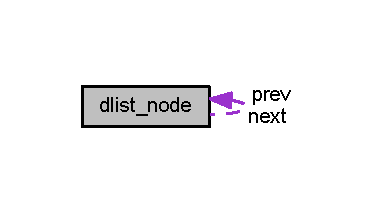
\includegraphics[width=179pt]{structdlist__node__coll__graph}
\end{center}
\end{figure}
\subsection*{Public Member Functions}
\begin{DoxyCompactItemize}
\item 
\hyperlink{structdlist__node_a2840ad5bcba6f82786afab43f775d81f}{dlist\-\_\-node} (int n)
\end{DoxyCompactItemize}
\subsection*{Public Attributes}
\begin{DoxyCompactItemize}
\item 
int \hyperlink{structdlist__node_abbcd93ff39230885440749f682aab79c}{d}
\item 
\hyperlink{structdlist__node}{dlist\-\_\-node} $\ast$ \hyperlink{structdlist__node_a446668c64b6554a885446e7766a0fca1}{next}
\item 
\hyperlink{structdlist__node}{dlist\-\_\-node} $\ast$ \hyperlink{structdlist__node_a63c2ec1d9d1d654ef30f01eb37ad5ff5}{prev}
\end{DoxyCompactItemize}


\subsection{Detailed Description}
Types of linked lists. 


\begin{DoxyEnumerate}
\item Linear linked lists
\item Circular linked lists.
\item Double linked lists.
\item Circular double linked lists.
\item others\-: xorlist 
\end{DoxyEnumerate}

Definition at line 16 of file list.\-h.



\subsection{Constructor \& Destructor Documentation}
\hypertarget{structdlist__node_a2840ad5bcba6f82786afab43f775d81f}{\index{dlist\-\_\-node@{dlist\-\_\-node}!dlist\-\_\-node@{dlist\-\_\-node}}
\index{dlist\-\_\-node@{dlist\-\_\-node}!dlist_node@{dlist\-\_\-node}}
\subsubsection[{dlist\-\_\-node}]{\setlength{\rightskip}{0pt plus 5cm}dlist\-\_\-node\-::dlist\-\_\-node (
\begin{DoxyParamCaption}
\item[{int}]{n}
\end{DoxyParamCaption}
)\hspace{0.3cm}{\ttfamily [inline]}}}\label{structdlist__node_a2840ad5bcba6f82786afab43f775d81f}


Definition at line 20 of file list.\-h.



\subsection{Member Data Documentation}
\hypertarget{structdlist__node_abbcd93ff39230885440749f682aab79c}{\index{dlist\-\_\-node@{dlist\-\_\-node}!d@{d}}
\index{d@{d}!dlist_node@{dlist\-\_\-node}}
\subsubsection[{d}]{\setlength{\rightskip}{0pt plus 5cm}int dlist\-\_\-node\-::d}}\label{structdlist__node_abbcd93ff39230885440749f682aab79c}


Definition at line 17 of file list.\-h.

\hypertarget{structdlist__node_a446668c64b6554a885446e7766a0fca1}{\index{dlist\-\_\-node@{dlist\-\_\-node}!next@{next}}
\index{next@{next}!dlist_node@{dlist\-\_\-node}}
\subsubsection[{next}]{\setlength{\rightskip}{0pt plus 5cm}{\bf dlist\-\_\-node}$\ast$ dlist\-\_\-node\-::next}}\label{structdlist__node_a446668c64b6554a885446e7766a0fca1}


Definition at line 18 of file list.\-h.

\hypertarget{structdlist__node_a63c2ec1d9d1d654ef30f01eb37ad5ff5}{\index{dlist\-\_\-node@{dlist\-\_\-node}!prev@{prev}}
\index{prev@{prev}!dlist_node@{dlist\-\_\-node}}
\subsubsection[{prev}]{\setlength{\rightskip}{0pt plus 5cm}{\bf dlist\-\_\-node}$\ast$ dlist\-\_\-node\-::prev}}\label{structdlist__node_a63c2ec1d9d1d654ef30f01eb37ad5ff5}


Definition at line 19 of file list.\-h.



The documentation for this struct was generated from the following file\-:\begin{DoxyCompactItemize}
\item 
Algo/\hyperlink{list_8h}{list.\-h}\end{DoxyCompactItemize}

\hypertarget{classsclist}{\section{sclist Class Reference}
\label{classsclist}\index{sclist@{sclist}}
}


A Circular Single Liked List with a head only.  




{\ttfamily \#include $<$list.\-h$>$}

\subsection*{Public Member Functions}
\begin{DoxyCompactItemize}
\item 
\hyperlink{classsclist_a22b47cdd2bea697d6e0b708a6fb904af}{sclist} ()
\item 
\hyperlink{classsclist_a82af11a92c4626a894dd98afbf4802cc}{sclist} (int $\ast$p, int $\ast$q)
\item 
\hyperlink{classsclist_aa3b32b45eb2d489f61a94002a720e5a7}{sclist} (int $\ast$p, int size)
\item 
\hyperlink{classsclist_a616510a8f7c9a6330e3f667e9fc35dcb}{sclist} (const vector$<$ int $>$ \&v)
\item 
\hyperlink{classsclist_a5eeb44634f2b0fbed000c1e303463881}{$\sim$sclist} ()
\item 
void \hyperlink{classsclist_ab18718668a0c9278922c1c173112aaee}{push\-\_\-front} (int n)
\begin{DoxyCompactList}\small\item\em push new node as the next of sentinel \end{DoxyCompactList}\item 
void \hyperlink{classsclist_a5646584dd15b375711c85343b88de3bf}{push\-\_\-front} (int $\ast$p, int $\ast$q)
\end{DoxyCompactItemize}


\subsection{Detailed Description}
A Circular Single Liked List with a head only. 

Definition at line 131 of file list.\-h.



\subsection{Constructor \& Destructor Documentation}
\hypertarget{classsclist_a22b47cdd2bea697d6e0b708a6fb904af}{\index{sclist@{sclist}!sclist@{sclist}}
\index{sclist@{sclist}!sclist@{sclist}}
\subsubsection[{sclist}]{\setlength{\rightskip}{0pt plus 5cm}sclist\-::sclist (
\begin{DoxyParamCaption}
{}
\end{DoxyParamCaption}
)}}\label{classsclist_a22b47cdd2bea697d6e0b708a6fb904af}
\hypertarget{classsclist_a82af11a92c4626a894dd98afbf4802cc}{\index{sclist@{sclist}!sclist@{sclist}}
\index{sclist@{sclist}!sclist@{sclist}}
\subsubsection[{sclist}]{\setlength{\rightskip}{0pt plus 5cm}sclist\-::sclist (
\begin{DoxyParamCaption}
\item[{int $\ast$}]{p, }
\item[{int $\ast$}]{q}
\end{DoxyParamCaption}
)}}\label{classsclist_a82af11a92c4626a894dd98afbf4802cc}
\hypertarget{classsclist_aa3b32b45eb2d489f61a94002a720e5a7}{\index{sclist@{sclist}!sclist@{sclist}}
\index{sclist@{sclist}!sclist@{sclist}}
\subsubsection[{sclist}]{\setlength{\rightskip}{0pt plus 5cm}sclist\-::sclist (
\begin{DoxyParamCaption}
\item[{int $\ast$}]{p, }
\item[{int}]{size}
\end{DoxyParamCaption}
)}}\label{classsclist_aa3b32b45eb2d489f61a94002a720e5a7}
\hypertarget{classsclist_a616510a8f7c9a6330e3f667e9fc35dcb}{\index{sclist@{sclist}!sclist@{sclist}}
\index{sclist@{sclist}!sclist@{sclist}}
\subsubsection[{sclist}]{\setlength{\rightskip}{0pt plus 5cm}sclist\-::sclist (
\begin{DoxyParamCaption}
\item[{const vector$<$ int $>$ \&}]{v}
\end{DoxyParamCaption}
)}}\label{classsclist_a616510a8f7c9a6330e3f667e9fc35dcb}
\hypertarget{classsclist_a5eeb44634f2b0fbed000c1e303463881}{\index{sclist@{sclist}!$\sim$sclist@{$\sim$sclist}}
\index{$\sim$sclist@{$\sim$sclist}!sclist@{sclist}}
\subsubsection[{$\sim$sclist}]{\setlength{\rightskip}{0pt plus 5cm}sclist\-::$\sim$sclist (
\begin{DoxyParamCaption}
{}
\end{DoxyParamCaption}
)}}\label{classsclist_a5eeb44634f2b0fbed000c1e303463881}


\subsection{Member Function Documentation}
\hypertarget{classsclist_ab18718668a0c9278922c1c173112aaee}{\index{sclist@{sclist}!push\-\_\-front@{push\-\_\-front}}
\index{push\-\_\-front@{push\-\_\-front}!sclist@{sclist}}
\subsubsection[{push\-\_\-front}]{\setlength{\rightskip}{0pt plus 5cm}void sclist\-::push\-\_\-front (
\begin{DoxyParamCaption}
\item[{int}]{n}
\end{DoxyParamCaption}
)}}\label{classsclist_ab18718668a0c9278922c1c173112aaee}


push new node as the next of sentinel 

\hypertarget{classsclist_a5646584dd15b375711c85343b88de3bf}{\index{sclist@{sclist}!push\-\_\-front@{push\-\_\-front}}
\index{push\-\_\-front@{push\-\_\-front}!sclist@{sclist}}
\subsubsection[{push\-\_\-front}]{\setlength{\rightskip}{0pt plus 5cm}void sclist\-::push\-\_\-front (
\begin{DoxyParamCaption}
\item[{int $\ast$}]{p, }
\item[{int $\ast$}]{q}
\end{DoxyParamCaption}
)}}\label{classsclist_a5646584dd15b375711c85343b88de3bf}


The documentation for this class was generated from the following file\-:\begin{DoxyCompactItemize}
\item 
Algo/\hyperlink{list_8h}{list.\-h}\end{DoxyCompactItemize}

\hypertarget{classslist}{\section{slist Class Reference}
\label{classslist}\index{slist@{slist}}
}


A H\-E\-A\-D\-\_\-\-T\-A\-I\-L Single Liked List with a head only.  




{\ttfamily \#include $<$list.\-h$>$}

\subsection*{Public Member Functions}
\begin{DoxyCompactItemize}
\item 
\hyperlink{classslist_aa8463ea4036bf8719f3faea241934858}{slist} ()
\item 
\hyperlink{classslist_a6a1a6479ec39a88e235c3571310ef275}{slist} (int $\ast$p, int $\ast$q)
\item 
\hyperlink{classslist_a37ec931ec2c1db1814e6e8bcb9940c59}{slist} (int $\ast$p, int size)
\item 
\hyperlink{classslist_a617a9bf75e1c3941ad1836cb168ec82b}{slist} (const vector$<$ int $>$ \&v)
\item 
\hyperlink{classslist_a4796fe87f2eb252c1d1b2ba7709cbe48}{$\sim$slist} ()
\item 
void \hyperlink{classslist_a40b17ed0d9449c5598d81275be700bb8}{push\-\_\-front} (int n)
\begin{DoxyCompactList}\small\item\em push new node as the next of sentinel \end{DoxyCompactList}\item 
void \hyperlink{classslist_abb64b3b995a604b62ab40a198ce4087c}{push\-\_\-front} (int $\ast$p, int $\ast$q)
\item 
\hyperlink{structslist__node}{slist\-\_\-node} $\ast$ \hyperlink{classslist_ae191f100c7bc3def2666f7164fa879a1}{end} ()
\item 
\hyperlink{structslist__node}{slist\-\_\-node} $\ast$ \hyperlink{classslist_af06c620ab7044adfe88f616b8df766b2}{begin} ()
\end{DoxyCompactItemize}
\subsection*{Static Public Member Functions}
\begin{DoxyCompactItemize}
\item 
static bool \hyperlink{classslist_a8cf488d289941111597ca79f1b45bfac}{test} ()
\end{DoxyCompactItemize}


\subsection{Detailed Description}
A H\-E\-A\-D\-\_\-\-T\-A\-I\-L Single Liked List with a head only. 

Definition at line 104 of file list.\-h.



\subsection{Constructor \& Destructor Documentation}
\hypertarget{classslist_aa8463ea4036bf8719f3faea241934858}{\index{slist@{slist}!slist@{slist}}
\index{slist@{slist}!slist@{slist}}
\subsubsection[{slist}]{\setlength{\rightskip}{0pt plus 5cm}slist\-::slist (
\begin{DoxyParamCaption}
{}
\end{DoxyParamCaption}
)}}\label{classslist_aa8463ea4036bf8719f3faea241934858}


Definition at line 4 of file slist.\-cpp.

\hypertarget{classslist_a6a1a6479ec39a88e235c3571310ef275}{\index{slist@{slist}!slist@{slist}}
\index{slist@{slist}!slist@{slist}}
\subsubsection[{slist}]{\setlength{\rightskip}{0pt plus 5cm}slist\-::slist (
\begin{DoxyParamCaption}
\item[{int $\ast$}]{p, }
\item[{int $\ast$}]{q}
\end{DoxyParamCaption}
)}}\label{classslist_a6a1a6479ec39a88e235c3571310ef275}


Definition at line 6 of file slist.\-cpp.



Here is the call graph for this function\-:
\nopagebreak
\begin{figure}[H]
\begin{center}
\leavevmode
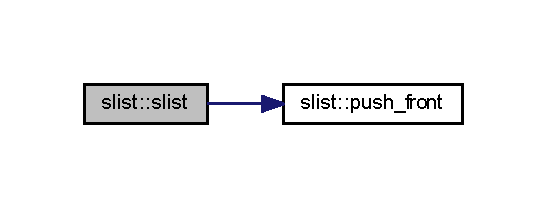
\includegraphics[width=262pt]{classslist_a6a1a6479ec39a88e235c3571310ef275_cgraph}
\end{center}
\end{figure}


\hypertarget{classslist_a37ec931ec2c1db1814e6e8bcb9940c59}{\index{slist@{slist}!slist@{slist}}
\index{slist@{slist}!slist@{slist}}
\subsubsection[{slist}]{\setlength{\rightskip}{0pt plus 5cm}slist\-::slist (
\begin{DoxyParamCaption}
\item[{int $\ast$}]{p, }
\item[{int}]{size}
\end{DoxyParamCaption}
)}}\label{classslist_a37ec931ec2c1db1814e6e8bcb9940c59}


Definition at line 11 of file slist.\-cpp.



Here is the call graph for this function\-:
\nopagebreak
\begin{figure}[H]
\begin{center}
\leavevmode
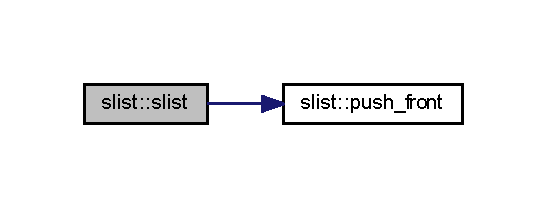
\includegraphics[width=262pt]{classslist_a37ec931ec2c1db1814e6e8bcb9940c59_cgraph}
\end{center}
\end{figure}


\hypertarget{classslist_a617a9bf75e1c3941ad1836cb168ec82b}{\index{slist@{slist}!slist@{slist}}
\index{slist@{slist}!slist@{slist}}
\subsubsection[{slist}]{\setlength{\rightskip}{0pt plus 5cm}slist\-::slist (
\begin{DoxyParamCaption}
\item[{const vector$<$ int $>$ \&}]{v}
\end{DoxyParamCaption}
)}}\label{classslist_a617a9bf75e1c3941ad1836cb168ec82b}


Definition at line 16 of file slist.\-cpp.

\hypertarget{classslist_a4796fe87f2eb252c1d1b2ba7709cbe48}{\index{slist@{slist}!$\sim$slist@{$\sim$slist}}
\index{$\sim$slist@{$\sim$slist}!slist@{slist}}
\subsubsection[{$\sim$slist}]{\setlength{\rightskip}{0pt plus 5cm}slist\-::$\sim$slist (
\begin{DoxyParamCaption}
{}
\end{DoxyParamCaption}
)}}\label{classslist_a4796fe87f2eb252c1d1b2ba7709cbe48}


Definition at line 18 of file slist.\-cpp.



\subsection{Member Function Documentation}
\hypertarget{classslist_af06c620ab7044adfe88f616b8df766b2}{\index{slist@{slist}!begin@{begin}}
\index{begin@{begin}!slist@{slist}}
\subsubsection[{begin}]{\setlength{\rightskip}{0pt plus 5cm}{\bf slist\-\_\-node} $\ast$ slist\-::begin (
\begin{DoxyParamCaption}
{}
\end{DoxyParamCaption}
)}}\label{classslist_af06c620ab7044adfe88f616b8df766b2}


Definition at line 39 of file slist.\-cpp.



Here is the caller graph for this function\-:
\nopagebreak
\begin{figure}[H]
\begin{center}
\leavevmode
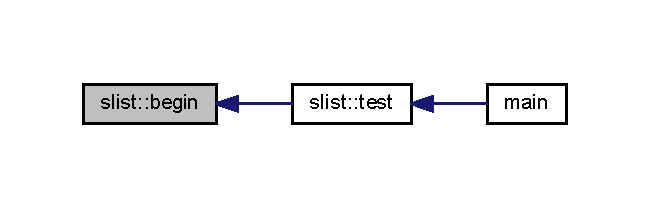
\includegraphics[width=312pt]{classslist_af06c620ab7044adfe88f616b8df766b2_icgraph}
\end{center}
\end{figure}


\hypertarget{classslist_ae191f100c7bc3def2666f7164fa879a1}{\index{slist@{slist}!end@{end}}
\index{end@{end}!slist@{slist}}
\subsubsection[{end}]{\setlength{\rightskip}{0pt plus 5cm}{\bf slist\-\_\-node} $\ast$ slist\-::end (
\begin{DoxyParamCaption}
{}
\end{DoxyParamCaption}
)}}\label{classslist_ae191f100c7bc3def2666f7164fa879a1}


Definition at line 35 of file slist.\-cpp.



Here is the caller graph for this function\-:
\nopagebreak
\begin{figure}[H]
\begin{center}
\leavevmode
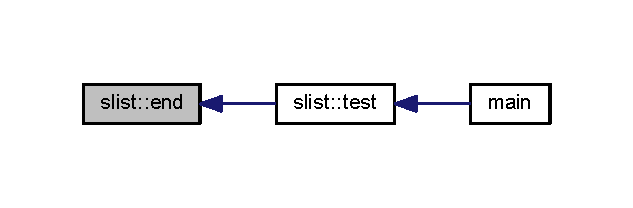
\includegraphics[width=304pt]{classslist_ae191f100c7bc3def2666f7164fa879a1_icgraph}
\end{center}
\end{figure}


\hypertarget{classslist_a40b17ed0d9449c5598d81275be700bb8}{\index{slist@{slist}!push\-\_\-front@{push\-\_\-front}}
\index{push\-\_\-front@{push\-\_\-front}!slist@{slist}}
\subsubsection[{push\-\_\-front}]{\setlength{\rightskip}{0pt plus 5cm}void slist\-::push\-\_\-front (
\begin{DoxyParamCaption}
\item[{int}]{n}
\end{DoxyParamCaption}
)}}\label{classslist_a40b17ed0d9449c5598d81275be700bb8}


push new node as the next of sentinel 



Definition at line 22 of file slist.\-cpp.



Here is the caller graph for this function\-:
\nopagebreak
\begin{figure}[H]
\begin{center}
\leavevmode
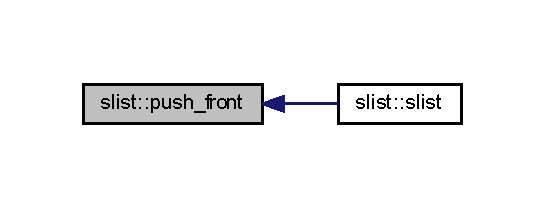
\includegraphics[width=262pt]{classslist_a40b17ed0d9449c5598d81275be700bb8_icgraph}
\end{center}
\end{figure}


\hypertarget{classslist_abb64b3b995a604b62ab40a198ce4087c}{\index{slist@{slist}!push\-\_\-front@{push\-\_\-front}}
\index{push\-\_\-front@{push\-\_\-front}!slist@{slist}}
\subsubsection[{push\-\_\-front}]{\setlength{\rightskip}{0pt plus 5cm}void slist\-::push\-\_\-front (
\begin{DoxyParamCaption}
\item[{int $\ast$}]{p, }
\item[{int $\ast$}]{q}
\end{DoxyParamCaption}
)}}\label{classslist_abb64b3b995a604b62ab40a198ce4087c}


Definition at line 33 of file slist.\-cpp.

\hypertarget{classslist_a8cf488d289941111597ca79f1b45bfac}{\index{slist@{slist}!test@{test}}
\index{test@{test}!slist@{slist}}
\subsubsection[{test}]{\setlength{\rightskip}{0pt plus 5cm}bool slist\-::test (
\begin{DoxyParamCaption}
{}
\end{DoxyParamCaption}
)\hspace{0.3cm}{\ttfamily [static]}}}\label{classslist_a8cf488d289941111597ca79f1b45bfac}


Definition at line 43 of file slist.\-cpp.



Here is the call graph for this function\-:
\nopagebreak
\begin{figure}[H]
\begin{center}
\leavevmode
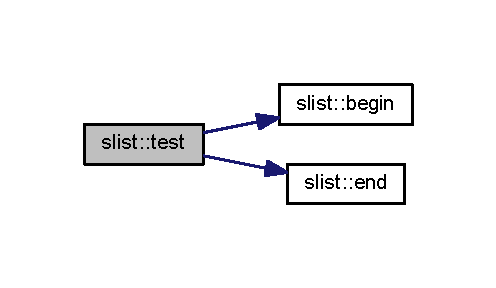
\includegraphics[width=238pt]{classslist_a8cf488d289941111597ca79f1b45bfac_cgraph}
\end{center}
\end{figure}




Here is the caller graph for this function\-:
\nopagebreak
\begin{figure}[H]
\begin{center}
\leavevmode
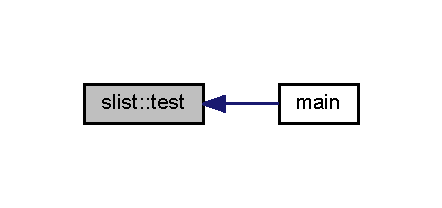
\includegraphics[width=212pt]{classslist_a8cf488d289941111597ca79f1b45bfac_icgraph}
\end{center}
\end{figure}




The documentation for this class was generated from the following files\-:\begin{DoxyCompactItemize}
\item 
Algo/\hyperlink{list_8h}{list.\-h}\item 
Algo/\hyperlink{slist_8cpp}{slist.\-cpp}\end{DoxyCompactItemize}

\hypertarget{structslist__node}{\section{slist\-\_\-node Struct Reference}
\label{structslist__node}\index{slist\-\_\-node@{slist\-\_\-node}}
}


{\ttfamily \#include $<$list.\-h$>$}



Collaboration diagram for slist\-\_\-node\-:
\nopagebreak
\begin{figure}[H]
\begin{center}
\leavevmode
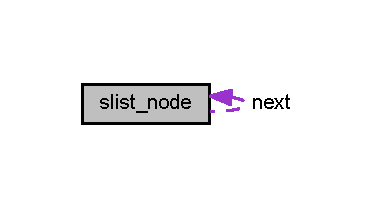
\includegraphics[width=180pt]{structslist__node__coll__graph}
\end{center}
\end{figure}
\subsection*{Public Member Functions}
\begin{DoxyCompactItemize}
\item 
\hyperlink{structslist__node_a07796f062d9bb5623c9ddaabcc46f009}{slist\-\_\-node} (int n)
\end{DoxyCompactItemize}
\subsection*{Public Attributes}
\begin{DoxyCompactItemize}
\item 
int \hyperlink{structslist__node_ad10237a1a1ad4ab70d89ad399e367cdc}{d}
\item 
\hyperlink{structslist__node}{slist\-\_\-node} $\ast$ \hyperlink{structslist__node_aee1e76b0000738d1bfda734232801359}{next}
\end{DoxyCompactItemize}


\subsection{Detailed Description}


Definition at line 97 of file list.\-h.



\subsection{Constructor \& Destructor Documentation}
\hypertarget{structslist__node_a07796f062d9bb5623c9ddaabcc46f009}{\index{slist\-\_\-node@{slist\-\_\-node}!slist\-\_\-node@{slist\-\_\-node}}
\index{slist\-\_\-node@{slist\-\_\-node}!slist_node@{slist\-\_\-node}}
\subsubsection[{slist\-\_\-node}]{\setlength{\rightskip}{0pt plus 5cm}slist\-\_\-node\-::slist\-\_\-node (
\begin{DoxyParamCaption}
\item[{int}]{n}
\end{DoxyParamCaption}
)\hspace{0.3cm}{\ttfamily [inline]}}}\label{structslist__node_a07796f062d9bb5623c9ddaabcc46f009}


Definition at line 100 of file list.\-h.



\subsection{Member Data Documentation}
\hypertarget{structslist__node_ad10237a1a1ad4ab70d89ad399e367cdc}{\index{slist\-\_\-node@{slist\-\_\-node}!d@{d}}
\index{d@{d}!slist_node@{slist\-\_\-node}}
\subsubsection[{d}]{\setlength{\rightskip}{0pt plus 5cm}int slist\-\_\-node\-::d}}\label{structslist__node_ad10237a1a1ad4ab70d89ad399e367cdc}


Definition at line 98 of file list.\-h.

\hypertarget{structslist__node_aee1e76b0000738d1bfda734232801359}{\index{slist\-\_\-node@{slist\-\_\-node}!next@{next}}
\index{next@{next}!slist_node@{slist\-\_\-node}}
\subsubsection[{next}]{\setlength{\rightskip}{0pt plus 5cm}{\bf slist\-\_\-node}$\ast$ slist\-\_\-node\-::next}}\label{structslist__node_aee1e76b0000738d1bfda734232801359}


Definition at line 99 of file list.\-h.



The documentation for this struct was generated from the following file\-:\begin{DoxyCompactItemize}
\item 
Algo/\hyperlink{list_8h}{list.\-h}\end{DoxyCompactItemize}

\chapter{File Documentation}
\hypertarget{bst_8cpp}{\section{Algo/bst.cpp File Reference}
\label{bst_8cpp}\index{Algo/bst.\-cpp@{Algo/bst.\-cpp}}
}
{\ttfamily \#include \char`\"{}bst.\-h\char`\"{}}\\*
{\ttfamily \#include $<$assert.\-h$>$}\\*
{\ttfamily \#include $<$iostream$>$}\\*
{\ttfamily \#include $<$stack$>$}\\*
{\ttfamily \#include $<$deque$>$}\\*
{\ttfamily \#include $<$set$>$}\\*
{\ttfamily \#include $<$iterator$>$}\\*
Include dependency graph for bst.\-cpp\-:\nopagebreak
\begin{figure}[H]
\begin{center}
\leavevmode
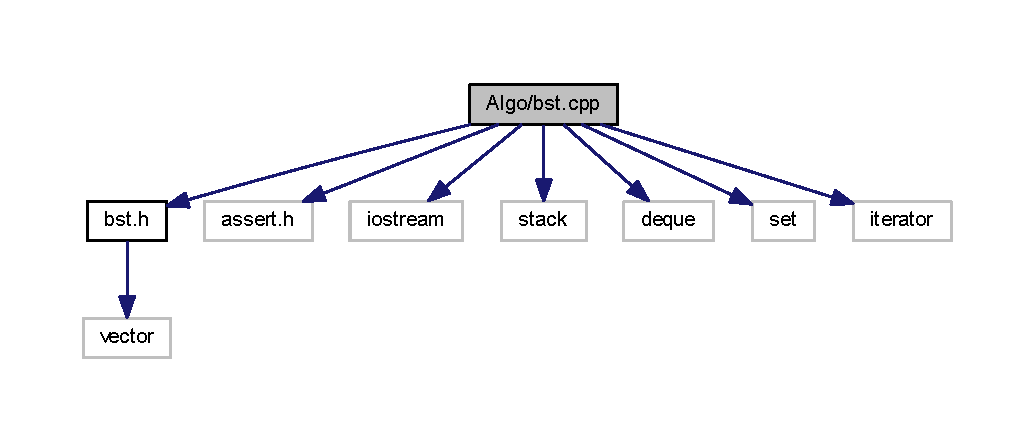
\includegraphics[width=350pt]{bst_8cpp__incl}
\end{center}
\end{figure}
\subsection*{Functions}
\begin{DoxyCompactItemize}
\item 
void \hyperlink{bst_8cpp_af9e41d3b82c0a62f7ab5e758526e43ff}{helper\-\_\-pushallleftsidenodes} (\hyperlink{structbtnode}{btnode} $\ast$b, stack$<$ \hyperlink{structbtnode}{btnode} $\ast$ $>$ \&s)
\item 
void \hyperlink{bst_8cpp_aec8339e67c16044cf6bfb738c589ee74}{helper\-\_\-pushallleftsidenodes} (\hyperlink{structbtnode}{btnode} $\ast$b, stack$<$ \hyperlink{structbtnode}{btnode} $\ast$ $>$ \&s, vector$<$ int $>$ \&v)
\item 
void \hyperlink{bst_8cpp_a198ad0345f981faef908c47735879645}{helper\-\_\-pushallrightsidenodes} (\hyperlink{structbtnode}{btnode} $\ast$b, stack$<$ \hyperlink{structbtnode}{btnode} $\ast$ $>$ \&s, vector$<$ int $>$ \&v)
\end{DoxyCompactItemize}


\subsection{Function Documentation}
\hypertarget{bst_8cpp_af9e41d3b82c0a62f7ab5e758526e43ff}{\index{bst.\-cpp@{bst.\-cpp}!helper\-\_\-pushallleftsidenodes@{helper\-\_\-pushallleftsidenodes}}
\index{helper\-\_\-pushallleftsidenodes@{helper\-\_\-pushallleftsidenodes}!bst.cpp@{bst.\-cpp}}
\subsubsection[{helper\-\_\-pushallleftsidenodes}]{\setlength{\rightskip}{0pt plus 5cm}void helper\-\_\-pushallleftsidenodes (
\begin{DoxyParamCaption}
\item[{{\bf btnode} $\ast$}]{b, }
\item[{stack$<$ {\bf btnode} $\ast$ $>$ \&}]{s}
\end{DoxyParamCaption}
)}}\label{bst_8cpp_af9e41d3b82c0a62f7ab5e758526e43ff}


Definition at line 104 of file bst.\-cpp.



Here is the caller graph for this function\-:
\nopagebreak
\begin{figure}[H]
\begin{center}
\leavevmode
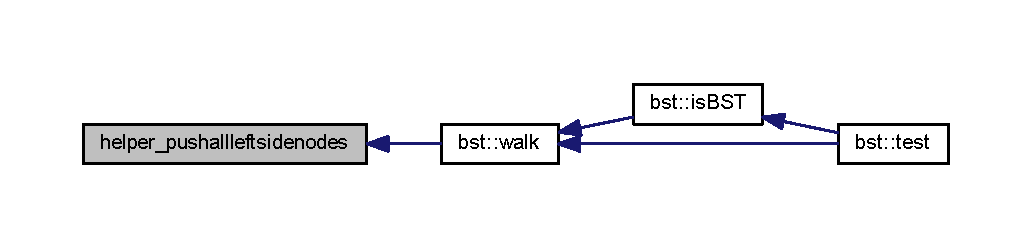
\includegraphics[width=350pt]{bst_8cpp_af9e41d3b82c0a62f7ab5e758526e43ff_icgraph}
\end{center}
\end{figure}


\hypertarget{bst_8cpp_aec8339e67c16044cf6bfb738c589ee74}{\index{bst.\-cpp@{bst.\-cpp}!helper\-\_\-pushallleftsidenodes@{helper\-\_\-pushallleftsidenodes}}
\index{helper\-\_\-pushallleftsidenodes@{helper\-\_\-pushallleftsidenodes}!bst.cpp@{bst.\-cpp}}
\subsubsection[{helper\-\_\-pushallleftsidenodes}]{\setlength{\rightskip}{0pt plus 5cm}void helper\-\_\-pushallleftsidenodes (
\begin{DoxyParamCaption}
\item[{{\bf btnode} $\ast$}]{b, }
\item[{stack$<$ {\bf btnode} $\ast$ $>$ \&}]{s, }
\item[{vector$<$ int $>$ \&}]{v}
\end{DoxyParamCaption}
)}}\label{bst_8cpp_aec8339e67c16044cf6bfb738c589ee74}


Definition at line 110 of file bst.\-cpp.

\hypertarget{bst_8cpp_a198ad0345f981faef908c47735879645}{\index{bst.\-cpp@{bst.\-cpp}!helper\-\_\-pushallrightsidenodes@{helper\-\_\-pushallrightsidenodes}}
\index{helper\-\_\-pushallrightsidenodes@{helper\-\_\-pushallrightsidenodes}!bst.cpp@{bst.\-cpp}}
\subsubsection[{helper\-\_\-pushallrightsidenodes}]{\setlength{\rightskip}{0pt plus 5cm}void helper\-\_\-pushallrightsidenodes (
\begin{DoxyParamCaption}
\item[{{\bf btnode} $\ast$}]{b, }
\item[{stack$<$ {\bf btnode} $\ast$ $>$ \&}]{s, }
\item[{vector$<$ int $>$ \&}]{v}
\end{DoxyParamCaption}
)}}\label{bst_8cpp_a198ad0345f981faef908c47735879645}


Definition at line 125 of file bst.\-cpp.



Here is the caller graph for this function\-:
\nopagebreak
\begin{figure}[H]
\begin{center}
\leavevmode
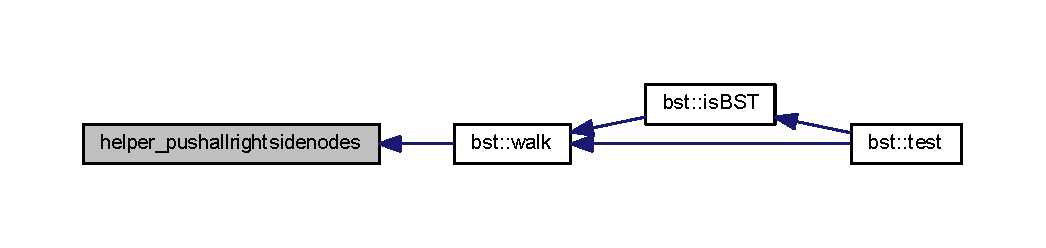
\includegraphics[width=350pt]{bst_8cpp_a198ad0345f981faef908c47735879645_icgraph}
\end{center}
\end{figure}



\hypertarget{bst_8h}{\section{Algo/bst.h File Reference}
\label{bst_8h}\index{Algo/bst.\-h@{Algo/bst.\-h}}
}
{\ttfamily \#include $<$vector$>$}\\*
Include dependency graph for bst.\-h\-:\nopagebreak
\begin{figure}[H]
\begin{center}
\leavevmode
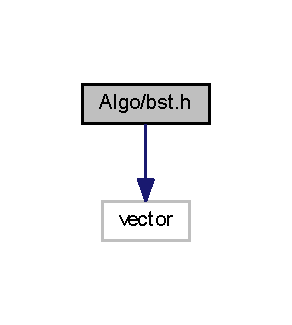
\includegraphics[width=140pt]{bst_8h__incl}
\end{center}
\end{figure}
This graph shows which files directly or indirectly include this file\-:\nopagebreak
\begin{figure}[H]
\begin{center}
\leavevmode
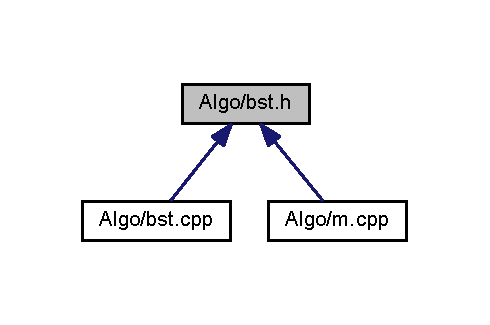
\includegraphics[width=235pt]{bst_8h__dep__incl}
\end{center}
\end{figure}
\subsection*{Classes}
\begin{DoxyCompactItemize}
\item 
struct \hyperlink{structbtnode}{btnode}
\begin{DoxyCompactList}\small\item\em arbitrary binary tree node\mbox{[}bst,heap,etc\mbox{]} \end{DoxyCompactList}\item 
class \hyperlink{classbt}{bt}
\begin{DoxyCompactList}\small\item\em an arbitrary binary tree \end{DoxyCompactList}\item 
class \hyperlink{classbst}{bst}
\begin{DoxyCompactList}\small\item\em an binary search tree \end{DoxyCompactList}\end{DoxyCompactItemize}
\subsection*{Enumerations}
\begin{DoxyCompactItemize}
\item 
enum \hyperlink{bst_8h_ae70daad8be95b143e7f97f55e1c4e743}{W\-A\-L\-K\-O\-R\-D\-E\-R} \{ \\*
\hyperlink{bst_8h_ae70daad8be95b143e7f97f55e1c4e743acd9d91cf59c093fdfa2b1736a26125ce}{P\-R\-E\-O\-R\-D\-E\-R} =1, 
\hyperlink{bst_8h_ae70daad8be95b143e7f97f55e1c4e743a541a7d029edbe0dc4855fa23ba23162b}{I\-N\-O\-R\-D\-E\-R}, 
\hyperlink{bst_8h_ae70daad8be95b143e7f97f55e1c4e743a9ab94412bf77ddc567d8cb5cd2996d44}{P\-O\-S\-T\-O\-R\-D\-E\-R}, 
\hyperlink{bst_8h_ae70daad8be95b143e7f97f55e1c4e743a5e981196031af46b1cfd4d0d34d19e26}{L\-A\-Y\-E\-R\-B\-Y\-L\-A\-Y\-E\-R}, 
\\*
\hyperlink{bst_8h_ae70daad8be95b143e7f97f55e1c4e743ad04285eca4b83d7798c137563d671341}{Z\-I\-G\-Z\-A\-G}, 
\hyperlink{bst_8h_ae70daad8be95b143e7f97f55e1c4e743ac157bdf0b85a40d2619cbc8bc1ae5fe2}{N\-O\-N\-E} =-\/1
 \}
\end{DoxyCompactItemize}


\subsection{Enumeration Type Documentation}
\hypertarget{bst_8h_ae70daad8be95b143e7f97f55e1c4e743}{\index{bst.\-h@{bst.\-h}!W\-A\-L\-K\-O\-R\-D\-E\-R@{W\-A\-L\-K\-O\-R\-D\-E\-R}}
\index{W\-A\-L\-K\-O\-R\-D\-E\-R@{W\-A\-L\-K\-O\-R\-D\-E\-R}!bst.h@{bst.\-h}}
\subsubsection[{W\-A\-L\-K\-O\-R\-D\-E\-R}]{\setlength{\rightskip}{0pt plus 5cm}enum {\bf W\-A\-L\-K\-O\-R\-D\-E\-R}}}\label{bst_8h_ae70daad8be95b143e7f97f55e1c4e743}
\begin{Desc}
\item[Enumerator]\par
\begin{description}
\index{P\-R\-E\-O\-R\-D\-E\-R@{P\-R\-E\-O\-R\-D\-E\-R}!bst.\-h@{bst.\-h}}\index{bst.\-h@{bst.\-h}!P\-R\-E\-O\-R\-D\-E\-R@{P\-R\-E\-O\-R\-D\-E\-R}}\item[{\em 
\hypertarget{bst_8h_ae70daad8be95b143e7f97f55e1c4e743acd9d91cf59c093fdfa2b1736a26125ce}{P\-R\-E\-O\-R\-D\-E\-R}\label{bst_8h_ae70daad8be95b143e7f97f55e1c4e743acd9d91cf59c093fdfa2b1736a26125ce}
}]\index{I\-N\-O\-R\-D\-E\-R@{I\-N\-O\-R\-D\-E\-R}!bst.\-h@{bst.\-h}}\index{bst.\-h@{bst.\-h}!I\-N\-O\-R\-D\-E\-R@{I\-N\-O\-R\-D\-E\-R}}\item[{\em 
\hypertarget{bst_8h_ae70daad8be95b143e7f97f55e1c4e743a541a7d029edbe0dc4855fa23ba23162b}{I\-N\-O\-R\-D\-E\-R}\label{bst_8h_ae70daad8be95b143e7f97f55e1c4e743a541a7d029edbe0dc4855fa23ba23162b}
}]\index{P\-O\-S\-T\-O\-R\-D\-E\-R@{P\-O\-S\-T\-O\-R\-D\-E\-R}!bst.\-h@{bst.\-h}}\index{bst.\-h@{bst.\-h}!P\-O\-S\-T\-O\-R\-D\-E\-R@{P\-O\-S\-T\-O\-R\-D\-E\-R}}\item[{\em 
\hypertarget{bst_8h_ae70daad8be95b143e7f97f55e1c4e743a9ab94412bf77ddc567d8cb5cd2996d44}{P\-O\-S\-T\-O\-R\-D\-E\-R}\label{bst_8h_ae70daad8be95b143e7f97f55e1c4e743a9ab94412bf77ddc567d8cb5cd2996d44}
}]\index{L\-A\-Y\-E\-R\-B\-Y\-L\-A\-Y\-E\-R@{L\-A\-Y\-E\-R\-B\-Y\-L\-A\-Y\-E\-R}!bst.\-h@{bst.\-h}}\index{bst.\-h@{bst.\-h}!L\-A\-Y\-E\-R\-B\-Y\-L\-A\-Y\-E\-R@{L\-A\-Y\-E\-R\-B\-Y\-L\-A\-Y\-E\-R}}\item[{\em 
\hypertarget{bst_8h_ae70daad8be95b143e7f97f55e1c4e743a5e981196031af46b1cfd4d0d34d19e26}{L\-A\-Y\-E\-R\-B\-Y\-L\-A\-Y\-E\-R}\label{bst_8h_ae70daad8be95b143e7f97f55e1c4e743a5e981196031af46b1cfd4d0d34d19e26}
}]\index{Z\-I\-G\-Z\-A\-G@{Z\-I\-G\-Z\-A\-G}!bst.\-h@{bst.\-h}}\index{bst.\-h@{bst.\-h}!Z\-I\-G\-Z\-A\-G@{Z\-I\-G\-Z\-A\-G}}\item[{\em 
\hypertarget{bst_8h_ae70daad8be95b143e7f97f55e1c4e743ad04285eca4b83d7798c137563d671341}{Z\-I\-G\-Z\-A\-G}\label{bst_8h_ae70daad8be95b143e7f97f55e1c4e743ad04285eca4b83d7798c137563d671341}
}]\index{N\-O\-N\-E@{N\-O\-N\-E}!bst.\-h@{bst.\-h}}\index{bst.\-h@{bst.\-h}!N\-O\-N\-E@{N\-O\-N\-E}}\item[{\em 
\hypertarget{bst_8h_ae70daad8be95b143e7f97f55e1c4e743ac157bdf0b85a40d2619cbc8bc1ae5fe2}{N\-O\-N\-E}\label{bst_8h_ae70daad8be95b143e7f97f55e1c4e743ac157bdf0b85a40d2619cbc8bc1ae5fe2}
}]\end{description}
\end{Desc}


Definition at line 26 of file bst.\-h.


\hypertarget{deque_8h}{\section{Algo/deque.h File Reference}
\label{deque_8h}\index{Algo/deque.\-h@{Algo/deque.\-h}}
}

\hypertarget{dlist_8cpp}{\section{Algo/dlist.cpp File Reference}
\label{dlist_8cpp}\index{Algo/dlist.\-cpp@{Algo/dlist.\-cpp}}
}
{\ttfamily \#include \char`\"{}list.\-h\char`\"{}}\\*
{\ttfamily \#include $<$iostream$>$}\\*
Include dependency graph for dlist.\-cpp\-:
\nopagebreak
\begin{figure}[H]
\begin{center}
\leavevmode
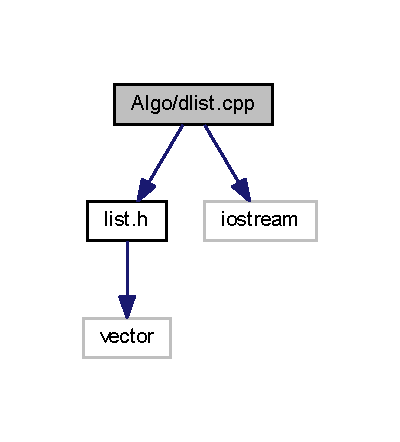
\includegraphics[width=192pt]{dlist_8cpp__incl}
\end{center}
\end{figure}

\hypertarget{dp_8h}{\section{Algo/dp.h File Reference}
\label{dp_8h}\index{Algo/dp.\-h@{Algo/dp.\-h}}
}

\hypertarget{heap_8h}{\section{Algo/heap.h File Reference}
\label{heap_8h}\index{Algo/heap.\-h@{Algo/heap.\-h}}
}

\hypertarget{htable_8h}{\section{Algo/htable.h File Reference}
\label{htable_8h}\index{Algo/htable.\-h@{Algo/htable.\-h}}
}

\hypertarget{list_8h}{\section{Algo/list.h File Reference}
\label{list_8h}\index{Algo/list.\-h@{Algo/list.\-h}}
}
{\ttfamily \#include $<$vector$>$}\\*
Include dependency graph for list.\-h\-:
\nopagebreak
\begin{figure}[H]
\begin{center}
\leavevmode
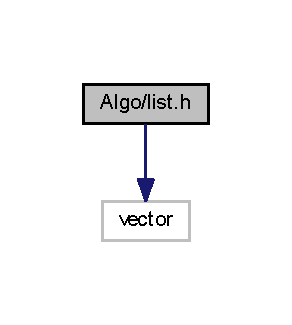
\includegraphics[width=140pt]{list_8h__incl}
\end{center}
\end{figure}
This graph shows which files directly or indirectly include this file\-:
\nopagebreak
\begin{figure}[H]
\begin{center}
\leavevmode
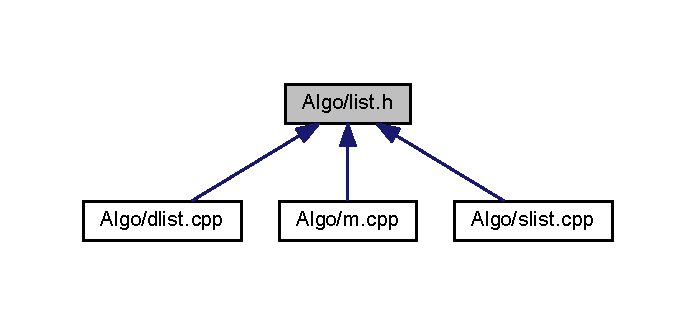
\includegraphics[width=334pt]{list_8h__dep__incl}
\end{center}
\end{figure}
\subsection*{Classes}
\begin{DoxyCompactItemize}
\item 
struct \hyperlink{structdlist__node}{dlist\-\_\-node}
\begin{DoxyCompactList}\small\item\em Types of linked lists. \end{DoxyCompactList}\item 
class \hyperlink{classdlist}{dlist}
\begin{DoxyCompactList}\small\item\em A H\-E\-A\-D\-\_\-\-T\-A\-I\-L Double Linked List. \end{DoxyCompactList}\item 
class \hyperlink{classdclist}{dclist}
\begin{DoxyCompactList}\small\item\em A Circular Double Linked List. \end{DoxyCompactList}\item 
struct \hyperlink{structslist__node}{slist\-\_\-node}
\item 
class \hyperlink{classslist}{slist}
\begin{DoxyCompactList}\small\item\em A H\-E\-A\-D\-\_\-\-T\-A\-I\-L Single Liked List with a head only. \end{DoxyCompactList}\item 
class \hyperlink{classsclist}{sclist}
\begin{DoxyCompactList}\small\item\em A Circular Single Liked List with a head only. \end{DoxyCompactList}\end{DoxyCompactItemize}

\hypertarget{m_8cpp}{\section{Algo/m.cpp File Reference}
\label{m_8cpp}\index{Algo/m.\-cpp@{Algo/m.\-cpp}}
}
{\ttfamily \#include $<$iostream$>$}\\*
{\ttfamily \#include $<$iterator$>$}\\*
{\ttfamily \#include \char`\"{}bst.\-h\char`\"{}}\\*
{\ttfamily \#include \char`\"{}list.\-h\char`\"{}}\\*
Include dependency graph for m.\-cpp\-:
\nopagebreak
\begin{figure}[H]
\begin{center}
\leavevmode
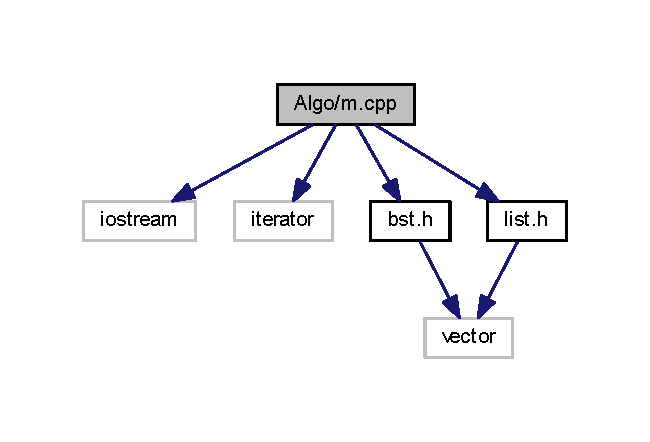
\includegraphics[width=312pt]{m_8cpp__incl}
\end{center}
\end{figure}
\subsection*{Functions}
\begin{DoxyCompactItemize}
\item 
int \hyperlink{m_8cpp_a0ddf1224851353fc92bfbff6f499fa97}{main} (int argc, char $\ast$argv\mbox{[}$\,$\mbox{]})
\end{DoxyCompactItemize}


\subsection{Function Documentation}
\hypertarget{m_8cpp_a0ddf1224851353fc92bfbff6f499fa97}{\index{m.\-cpp@{m.\-cpp}!main@{main}}
\index{main@{main}!m.cpp@{m.\-cpp}}
\subsubsection[{main}]{\setlength{\rightskip}{0pt plus 5cm}int main (
\begin{DoxyParamCaption}
\item[{int}]{argc, }
\item[{char $\ast$}]{argv\mbox{[}$\,$\mbox{]}}
\end{DoxyParamCaption}
)}}\label{m_8cpp_a0ddf1224851353fc92bfbff6f499fa97}


Definition at line 8 of file m.\-cpp.



Here is the call graph for this function\-:
\nopagebreak
\begin{figure}[H]
\begin{center}
\leavevmode
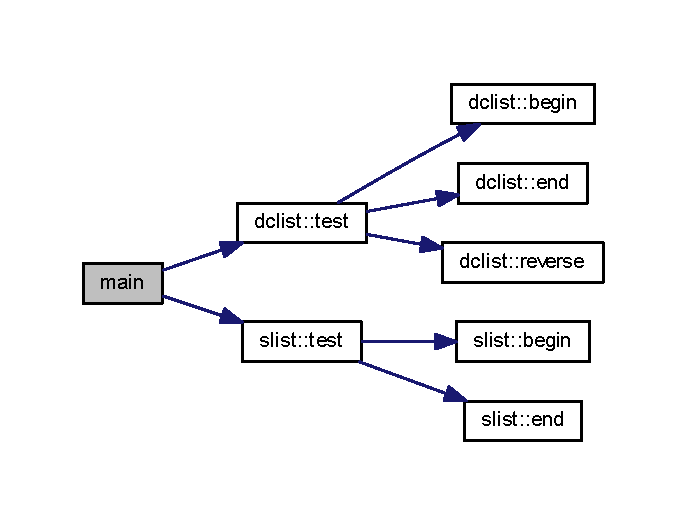
\includegraphics[width=330pt]{m_8cpp_a0ddf1224851353fc92bfbff6f499fa97_cgraph}
\end{center}
\end{figure}



\hypertarget{queue_8h}{\section{Algo/queue.h File Reference}
\label{queue_8h}\index{Algo/queue.\-h@{Algo/queue.\-h}}
}

\hypertarget{slist_8cpp}{\section{Algo/slist.cpp File Reference}
\label{slist_8cpp}\index{Algo/slist.\-cpp@{Algo/slist.\-cpp}}
}
{\ttfamily \#include \char`\"{}list.\-h\char`\"{}}\\*
{\ttfamily \#include $<$iostream$>$}\\*
Include dependency graph for slist.\-cpp\-:
\nopagebreak
\begin{figure}[H]
\begin{center}
\leavevmode
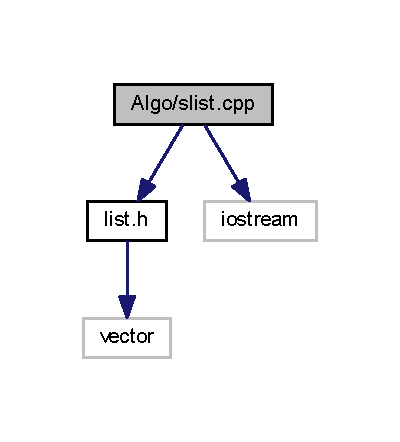
\includegraphics[width=192pt]{slist_8cpp__incl}
\end{center}
\end{figure}

\hypertarget{stack_8h}{\section{Algo/stack.h File Reference}
\label{stack_8h}\index{Algo/stack.\-h@{Algo/stack.\-h}}
}

\hypertarget{util_8h}{\section{Algo/util.h File Reference}
\label{util_8h}\index{Algo/util.\-h@{Algo/util.\-h}}
}

%--- End generated contents ---

% Index
\newpage
\phantomsection
\addcontentsline{toc}{part}{Index}
\printindex

\end{document}
